\documentclass[11pt]{article}

% ---------------------------------------------------------------------------
% Overleaf-ready. Compiles with pdfLaTeX (Overleaf default) or Tectonic.
% Only standard, widely available packages are used.
% ---------------------------------------------------------------------------
\usepackage[utf8]{inputenc}
\usepackage[T1]{fontenc}
\usepackage[a4paper,margin=1in]{geometry}
\usepackage{amsmath,amssymb,amsthm}
\usepackage{booktabs}
\usepackage{multirow}
\usepackage{graphicx}
\usepackage{xcolor}
\usepackage{microtype}
\usepackage{enumitem}
\usepackage[hidelinks]{hyperref}
\usepackage{caption}
\usepackage{tikz}
\usetikzlibrary{arrows.meta,positioning,fit,calc,backgrounds,shapes.geometric}
\usepackage{pgfplots}
\pgfplotsset{compat=1.16}
\usepgfplotslibrary{groupplots}
\usepackage{algorithm}
\usepackage{algpseudocode}
\captionsetup{font=small,labelfont=bf}

\newtheorem{definition}{Definition}
\newtheorem{proposition}{Proposition}

\newcommand{\Cmax}{C_{\max}}
\newcommand{\R}{\mathbb{R}}
\newcommand{\argmax}{\operatorname*{arg\,max}}
\DeclareMathOperator{\softmax}{softmax}
\DeclareMathOperator{\LeakyReLU}{LeakyReLU}
\DeclareMathOperator{\ReLU}{ReLU}
\DeclareMathOperator{\MLP}{MLP}
\DeclareMathOperator*{\maxop}{max}
\newcommand{\concat}{\,\Vert\,}

% TikZ styles for the architecture / DAG diagrams
\tikzset{
  blk/.style={draw, rounded corners=2pt, align=center, inner sep=4pt, font=\footnotesize},
  core/.style={blk, fill=blue!8},
  head/.style={blk, fill=green!8},
  io/.style={blk, fill=gray!8},
  ev/.style={draw, circle, minimum size=15pt, inner sep=0pt, font=\scriptsize},
  crit/.style={very thick, red},
  fl/.style={-{Latex[length=2mm]}},
}

\title{\textbf{Faithful Tropical Explanations for Guiding\\[2pt]
Bi-Objective Quay-Crane and Speed-Adjustable-AGV Scheduling}}

\author{Aayush Jha}
\date{\today}

\begin{document}
\maketitle

\begin{abstract}
\noindent
This paper treats the bi-objective scheduling of quay cranes (QCs) and speed-adjustable
automated guided vehicles (SA-AGVs) in a dual-cycling container terminal, where the two
competing objectives are the makespan $\Cmax$ and the total AGV travel energy $E$. The
reference method is the multi-population biased random-key genetic algorithm (mp-BRKGA)
of Fontes and Homayouni. The question addressed is whether an explanation of why a
schedule is good can be made faithful enough to describe the behaviour of the Pareto
front and to steer the search.
The model introduced here is a physics-fused heterogeneous graph attention surrogate
(E-HGATv2) whose makespan is produced by an exact max-plus (tropical) longest-path layer.
Because the makespan flows through the critical-path recurrence itself, the network's
gradient with respect to each transport leg is an exact binary critical-path indicator;
this readout is denoted TAPE (Tropical Attribution for Physical Explanations). On $11$
problem instances (synthetic dual-cycling instances and the published FSMJ loading
benchmark, in both the uncoupled and the peak-power-coupled regime) TAPE recovers the
true critical path with Jaccard $0.85$--$1.00$ against the exact evaluator, whereas the
learned attention weights are statistically uncorrelated with the true makespan levers
($|\rho|\le 0.18$) and, measured against the exact critical path from coarse hit-rate to
fine ranking, are no better than random at any granularity. Routing the same signal back
into an NSGA-II search makes the guided algorithm dominate mp-BRKGA, single-population
BRKGA and an unguided control on hypervolume in $11/11$ instances (Friedman
$\chi^2_4=35.1$, $p=4.5\times10^{-7}$; all post-hoc Holm-adjusted $p\le0.004$).
Aggregating TAPE over the approximated Pareto set with a trade-off-weighted score
(Trade-off Criticality Score) yields a sparse description of how the binding bottleneck
migrates along the front, and a single structural surrogate transfers this front
composition to unseen instances (Pearson $r=0.945$ on a composition-spanning set). The
same mathematical object thus explains the front, characterises its behaviour, and guides
the optimiser.
\end{abstract}

\section{Introduction}
\label{sec:intro}

The container terminal scheduling problem treated here couples three decisions:
assignment of container moves (tasks) to vehicles, sequencing of tasks on each vehicle
and on each crane, and the speed level of every vehicle leg, which trades travel time
against energy. Two objectives are minimised, the makespan $\Cmax$ and the total travel
energy $E$. The reference method is the multi-population biased random-key genetic
algorithm (mp-BRKGA) of Fontes and Homayouni~\cite{fontes2022mpbrkga}.

Four questions arise in this setting and are treated together here. Which quantities
drive the objectives, as recovered by post-hoc analysis of solved instances? Why is a
given solution Pareto-optimal, expressed in terms of the input variables (task order,
vehicle speed, crane workload)? Can knowledge gathered during the search steer the
optimiser, in the sense of selecting which neighbourhood to explore and which operator to
apply? And can that knowledge be extracted in a form that characterises the Pareto front
rather than a single schedule?

A single mathematical object addresses all four: the gradient of an exact max-plus
longest path embedded inside a learned surrogate. It serves as a post-hoc importance
signal over the input variables, as a steering signal fed back to NSGA-II, and,
aggregated over the front with a trade-off weight, as a description of front behaviour.
The requirement throughout is faithfulness in a specific sense, that the signal identify
the operations which set the makespan rather than produce a plausible-looking heat map.
Learned attention weights read directly as explanations do not meet that requirement in
this problem, and Section~\ref{sec:results} quantifies the gap.

\section{Problem formulation}
\label{sec:problem}

\subsection{Entities and decisions}
An instance has a set of container moves (\emph{tasks}) $\mathcal{J}=\{0,\dots,N-1\}$.
Each task $j$ is bound to one quay crane $\mathrm{qc}(j)$ and one yard/storage station
$\mathrm{lu}(j)$, and is of one of two kinds: a \emph{LOAD} (export: the loaded vehicle leg
runs $\mathrm{LU}\!\to\!\mathrm{QC}$) or an \emph{UNLOAD} (import: the loaded leg runs
$\mathrm{QC}\!\to\!\mathrm{LU}$). Each crane processes its tasks one at a time with a
handling time $\tau_j$. A fleet of $|\mathcal{A}|$ SA-AGVs performs the transport. A
decision specifies, for every task, (a) the assigned vehicle, (b) the position in that
vehicle's sequence and in its crane's sequence, and (c) a discrete speed level for the
\emph{empty} leg (vehicle driving to the pickup) and for the \emph{loaded} leg.

\subsection{Physics of a leg}
Three speed levels $\alpha\in\{0.8,1.0,1.2\}$ scale a nominal speed; loaded and empty legs
have distinct nominal speeds and power draws (Table~\ref{tab:speed}, after
\cite{homayouni2022book,fontes2022mpbrkga}). For a leg of length $d$ at level $\ell$,
\begin{equation}
t_{\text{leg}}(d,\ell) = \frac{d}{v_\ell}, \qquad
e_{\text{leg}}(d,\ell) = P_\ell \cdot t_{\text{leg}}(d,\ell),
\end{equation}
i.e.\ energy is power $\times$ time. A faster level shortens $t$ but raises $P$, which is
the source of the time--energy trade-off.

\begin{table}[t]
\centering
\caption{Kinematic and power constants per speed level (after \cite{homayouni2022book}).}
\label{tab:speed}
\small
\resizebox{\textwidth}{!}{%
\begin{tabular}{lccccc}
\toprule
Level & $\alpha$ & empty $v$ (m/s) & empty $P$ (kW) & loaded $v$ (m/s) & loaded $P$ (kW)\\
\midrule
Lower   & 0.8 & 4.8 & 7.8  & 2.4 & 11.7\\
Nominal & 1.0 & 6.0 & 10.0 & 3.0 & 15.0\\
Higher  & 1.2 & 7.2 & 13.2 & 3.6 & 19.8\\
\bottomrule
\end{tabular}}
\end{table}

\subsection{Objectives and the max-plus structure of the makespan}
\label{sec:maxplus}
Total energy is simply additive over the chosen legs,
\begin{equation}
E \;=\; \sum_{j\in\mathcal{J}} \big(e^{\text{empty}}_j + e^{\text{loaded}}_j\big).
\label{eq:energy}
\end{equation}
The makespan is more subtle. Fixing the assignment and sequencing turns the schedule into a
\emph{precedence graph}: task $j$ cannot start its work until both its predecessor on the
same vehicle and its predecessor on the same crane have finished. Following the corrected
single-indexed timing of \cite{fontes2023flowtime}, the per-task completion obeys, for a
LOAD,
\begin{equation}
c_j \;=\; \max\!\big(a^{\text{agv}}_j + t^{\text{empty}}_j + t^{\text{loaded}}_j,\;
c_{\mathrm{qcprev}(j)}\big) + \tau_j ,
\end{equation}
and for an UNLOAD,
\begin{equation}
c_j \;=\; \max\!\big(a^{\text{agv}}_j + t^{\text{empty}}_j,\; c_{\mathrm{qcprev}(j)} + \tau_j\big)
+ t^{\text{loaded}}_j ,
\end{equation}
with $a^{\text{agv}}_j$ the time the vehicle becomes free for $j$. Because every completion
is a \emph{maximum of sums} along the vehicle and crane chains, the makespan
\begin{equation}
\Cmax \;=\; \max_{j} c_j
\end{equation}
is exactly a \emph{longest path} in the precedence graph under the algebra
$(\max,+)$---the \emph{tropical} or \emph{max-plus} semiring~\cite{baccelli1992synch}. This
is the single structural fact the whole method exploits: the longest path is the
\emph{critical path}, and the objective is determined by the activities lying on it.

\subsection{The peak-power-coupled regime}
\label{sec:coupled}
The uncoupled problem above has a closed-form (longest-path) makespan. As a deliberately
harder, \emph{no-closed-form} stress-test for the differentiable surrogate, we add a
constraint of our own construction: the fleet shares a single \emph{instantaneous peak-power
budget} $P_{\max}$, and the total power of all AGV \emph{travel legs} running at any instant
may not exceed $P_{\max}$ (quay-crane handling draws none). Any
$P_{\max}\ge\max_\ell \varepsilon_\ell$ ($=19.8$\,kW from Table~\ref{tab:speed}; we use
$30$\,kW) keeps every leg individually feasible.

\paragraph{Activity model.} Each task $j$ expands into power-drawing legs and zero-power
timing nodes whose precedence \emph{reproduces the uncoupled recurrence of
Section~\ref{sec:maxplus} exactly}. The empty (E) and loaded (L) legs draw power
$e_\ell,\varepsilon_\ell$ for their durations $t^{\mathrm e}_j,t^{\mathrm l}_j$; the
zero-duration nodes are the AGV release R (at the quay pickup, for a LOAD) and the completion
C (for an UNLOAD), and node H carries the handling time $\tau_j$. Within a task the order is
$\mathrm{E}\!\to\!\mathrm{L}\!\to\!\mathrm{R}\!\to\!\mathrm{H}$ (LOAD) or
$\mathrm{E}\!\to\!\mathrm{C}\!\to\!\mathrm{L}$ (UNLOAD), with R/C gated by the crane chain so
that, \emph{absent the cap}, the realised completions equal the closed-form $c_j$ of
Eqs.~(LOAD/UNLOAD); AGV- and crane-chain arcs link consecutive tasks.

\paragraph{Resolution.} A power leg may \emph{start} only once its precedence is met
and starting it keeps the sum of concurrently-running leg powers $\le P_{\max}$;
otherwise it waits for a running leg to finish and free budget. The schedule is realised by a
deterministic \emph{parallel schedule-generation scheme}: at each completion event, ready legs
are started greedily in priority order---earliest available, then task index, then
empty-before-loaded---until the budget is exhausted. This makes $(\Cmax,E)$ a
\emph{well-defined, exact} function of the decision $z$ (energy is unchanged, being
timing-independent), but the makespan is \emph{no longer} a max-plus longest path: the cap
injects disjunctive \emph{power-wait} arcs (a blocker leg $\to$ the leg it delays) that no
closed form captures. When $P_{\max}$ is large enough that no leg ever waits, the scheme
provably reduces to the uncoupled evaluator (a unit test asserts this), so the coupled problem
is a clean \emph{superset} of the validated uncoupled one.

\paragraph{Scope of the construction.} Two limitations delimit this regime. \emph{(i)} The power
arbitration is a \emph{fixed dispatch policy} (the priority rule above) rather than a decision
variable; the regime optimises the assignment, order and speeds under that policy.
\emph{(ii)} Unlike the uncoupled objective---the published recurrence~\cite{fontes2023flowtime},
validated against the exact evaluator---the coupled constraint is introduced in this work: it does
not form part of the FSMJ or book-chapter benchmark, and we make no claim that it models a
specific installation. Its role is methodological. It is the regime in which the makespan admits
no closed form and the binding leg is not evident by inspection, and therefore the regime in
which a differentiable surrogate with exact gradients (TAPE) is required; accordingly, the fused
head carries an explicit power-wait term (Section~\ref{sec:fused}).

\section{Method}
\label{sec:method}

\paragraph{Overview.} There is no labelled training corpus. An exact
simulator---the \emph{evaluator} (Section~\ref{sec:evaluator})---scores any candidate schedule
and, as a by-product, emits the duration of every transport leg; a graph network then learns
to imitate those durations. Concretely (Figure~\ref{fig:arch}): a search proposal is decoded
into a feasible schedule (Section~\ref{sec:randomkey}), recast as a heterogeneous graph
(Section~\ref{sec:graphrep}) and embedded by the E-HGATv2 surrogate (Section~\ref{sec:ehgat});
projection heads predict each leg's duration, which an \emph{exact} max-plus dynamic program
(Section~\ref{sec:fused}) recomposes into the makespan. Because the makespan flows through the
genuine critical-path recurrence, differentiating it returns an \emph{exact} indicator of
which operations bind the schedule---the TAPE explanation (Section~\ref{sec:tape}). That same
signal biases the search's variation operators and screens its offspring
(Section~\ref{sec:guidance}) and, aggregated over the Pareto front, describes how the binding
bottleneck migrates (Section~\ref{sec:pts}). The rest of this section dissects each block with
the notation of Table~\ref{tab:notation}.

\subsection{Decision variables and the search space}
\label{sec:searchspace}
An instance has $N$ transport tasks $\mathcal{J}=\{1,\dots,N\}$, a fleet of $A$
speed-adjustable AGVs, $K$ quay cranes, and $V$ admissible speed levels per leg. A
\emph{solution} is the tuple
\begin{equation}
z \;=\; \big(\,\alpha,\;\sigma,\;\omega^{\mathrm e},\;\omega^{\mathrm l}\,\big),\qquad
\alpha:\mathcal{J}\!\to\!\{1,\dots,A\},\;\;
\sigma\in\mathfrak{S}_N,\;\;
\omega^{\mathrm e},\omega^{\mathrm l}\in\{1,\dots,V\}^{N},
\label{eq:solution}
\end{equation}
i.e.\ an assignment $\alpha$ of each task to a vehicle, a processing order $\sigma$, and a
speed level for each empty (e) and loaded (l) leg. The decoder of
Section~\ref{sec:randomkey} turns $z$ into a feasible schedule $s(z)$ whose physical
evaluation returns the objective pair $f(s)=(\Cmax(s),E(s))$. The cardinality of the
feasible set,
\begin{equation}
|\mathcal{Z}| \;=\; \underbrace{A^{N}}_{\text{assignment}}\cdot
\underbrace{N!}_{\text{order}}\cdot
\underbrace{V^{2N}}_{\text{speeds}},
\end{equation}
grows super-exponentially (already $>10^{40}$ at $N{=}20$, $A{=}3$, $V{=}3$), and the
underlying assignment--sequencing problem is NP-hard~\cite{fontes2022mpbrkga}; exact MILP is
intractable beyond a few dozen tasks. We therefore search with the population-based
metaheuristic NSGA-II~\cite{deb2002nsga2} and concentrate our contribution on where
in $\mathcal Z$ the search spends its budget: a faithful, physics-anchored explanation of
\emph{which decisions bind the objectives} is used to bias the variation operators and to
screen offspring (Sections~\ref{sec:guidance}).

\begin{table}[t]
\centering\small
\caption{Notation used throughout the Method.}
\label{tab:notation}
\begin{tabular}{@{}ll@{}}
\toprule
Symbol & Meaning\\
\midrule
$\mathcal J=\{1,\dots,N\}$ & transport tasks\\
$A,\,K,\,V$ & \# AGVs, \# quay cranes, \# speed levels per leg\\
$z=(\alpha,\sigma,\omega^{\mathrm e},\omega^{\mathrm l})$ & a solution (Eq.~\ref{eq:solution})\\
$s(z)$, $f(s)=(\Cmax,E)$ & decoded schedule and its objective pair\\
$G_s=(\mathcal V,\,E^{\mathrm{agv}},E^{\mathrm{qc}})$ & heterogeneous schedule graph\\
$x_j\in\R^{d_0}$, $u_{ij}\in\R^{d_e}$ & task-node and arc input features\\
$h_j^{(\ell)}\in\R^{d}$ & embedding of task $j$ after layer $\ell$\\
$\mathcal N_r(j)$ & resource-$r$ predecessors of $j$ ($r\in\{\mathrm{agv},\mathrm{qc}\}$)\\
$\beta_j^{r}$ & semantic (cross-resource) attention of $j$ on $r$\\
$t^{\mathrm e}_j,t^{\mathrm l}_j$ & empty/loaded leg times of task $j$\\
$e^{\mathrm e}_j,e^{\mathrm l}_j$ & empty/loaded leg energies of task $j$ ($E=\sum_j e^{\mathrm e}_j+e^{\mathrm l}_j$)\\
$\tau_j$ & crane handling delay of task $j$\\
$M$ & \# sampled schedules used to train the surrogate\\
$G_{\mathrm{dag}}=(\mathcal N,\mathcal A,b,w)$ & event DAG: node weights $b$, arc weights $w$\\
$\pi^\star$ & critical (longest) path in $G_{\mathrm{dag}}$\\
$g_a=\partial\Cmax/\partial w_a$ & TAPE attribution of arc $a$\\
\bottomrule
\end{tabular}
\end{table}

\subsection{Random-key representation and the decoder}
\label{sec:randomkey}
We use the biased random-key encoding~\cite{fontes2022mpbrkga}: a chromosome is a vector
$\chi\in[0,1]^{4N}$ split into four length-$N$ blocks. The deterministic decoder
$\mathcal D:[0,1]^{4N}\!\to\!\mathcal Z$ reads task order from the argsort of the first
block, vehicle assignment from $\lceil A\,\chi^{(2)}\rceil$, and the two speed levels from
$\lceil V\,\chi^{(3)}\rceil,\lceil V\,\chi^{(4)}\rceil$; structural feasibility (one vehicle
per task, crane order from the fixed bay layout) is enforced during decoding. The optimiser
is elitist NSGA-II~\cite{deb2002nsga2}; our contribution lies in \emph{how its mutation and
screening are guided}.

\begin{figure}[t]
\centering
\resizebox{\textwidth}{!}{%
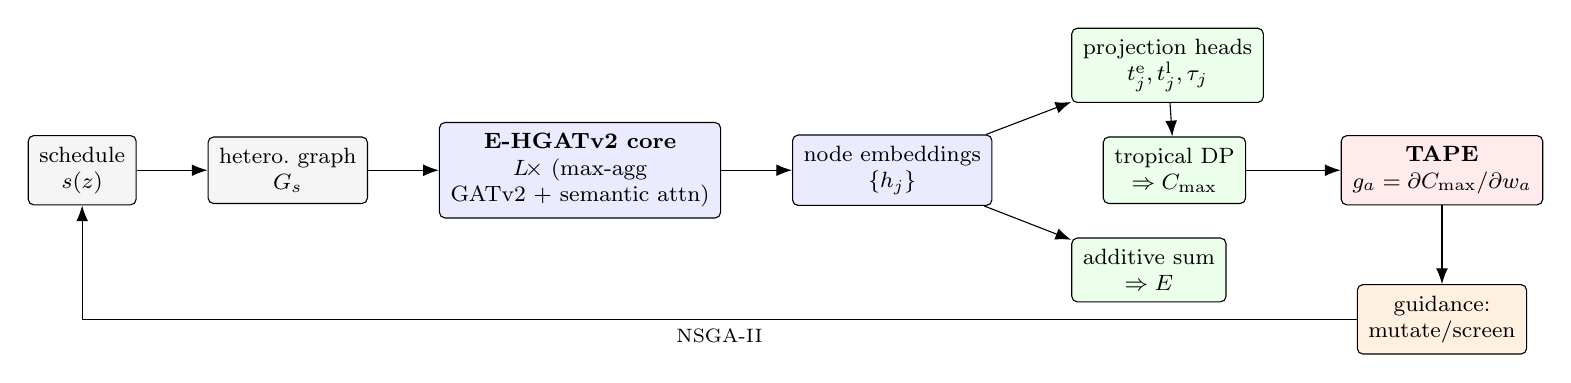
\begin{tikzpicture}[node distance=6mm and 9mm]
\node[io] (sched) {schedule\\$s(z)$};
\node[io, right=of sched] (graph) {hetero.\ graph\\$G_s$};
\node[core, right=of graph] (core) {\textbf{E-HGATv2 core}\\$L\!\times$ (max-agg\\GATv2 $+$ semantic attn)};
\node[core, right=of core] (emb) {node embeddings\\$\{h_j\}$};
\node[head, above right=4mm and 10mm of emb] (proj) {projection heads\\$t^{\mathrm e}_j,t^{\mathrm l}_j,\tau_j$};
\node[head, right=14mm of emb] (dp) {tropical DP\\$\Rightarrow \Cmax$};
\node[head, below right=4mm and 10mm of emb] (en) {additive sum\\$\Rightarrow E$};
\node[blk, fill=red!8, right=12mm of dp] (tape) {\textbf{TAPE}\\$g_a=\partial\Cmax/\partial w_a$};
\node[blk, fill=orange!12, below=10mm of tape] (guide) {guidance:\\mutate/screen};
\draw[fl] (sched)--(graph);
\draw[fl] (graph)--(core);
\draw[fl] (core)--(emb);
\draw[fl] (emb)--(proj);
\draw[fl] (emb)--(en);
\draw[fl] (proj)--(dp);
\draw[fl] (dp)--(tape);
\draw[fl] (tape)--(guide);
\draw[fl] (guide) -| node[pos=0.25,below,font=\scriptsize]{NSGA-II} (sched);
\end{tikzpicture}%
}
\caption{Pipeline. The E-HGATv2 core embeds a decoded schedule; projection heads predict
local physical attributes that an \emph{exact} max-plus dynamic program composes into
$\Cmax$ (energy is an exact additive sum). Differentiating the DP yields the TAPE arc
attributions $g_a$, which both \emph{explain} the schedule and \emph{steer} the next NSGA-II
generation.}
\label{fig:arch}
\end{figure}

\subsection{Heterogeneous graph representation of a schedule}
\label{sec:graphrep}
A decoded schedule $s(z)$ is encoded as a directed heterogeneous graph
$G_s=(\mathcal V,E^{\mathrm{agv}},E^{\mathrm{qc}})$ in which every transport task is a node $j\in\mathcal V$
and the two resource chains are the two arc types:
\begin{itemize}[leftmargin=*,itemsep=2pt]
  \item a \textbf{task-node feature} $x_j\in\R^{d_0}$, $d_0{=}4$, holds the handling time,
  task kind and origin/\allowbreak destination descriptors;
  \item an \textbf{AGV arc} $(i\!\to\! j)\in E^{\mathrm{agv}}$ exists iff task $i$ is the
  immediate vehicle-predecessor of $j$ under $\alpha,\sigma$; its feature
  $u_{ij}\in\R^{d_e}$ ($d_e{=}3$) carries the leg travel time and the empty/loaded leg
  energies;
  \item a \textbf{QC arc} $(i\!\to\! j)\in E^{\mathrm{qc}}$ exists iff $i$ immediately
  precedes $j$ on the same crane.
\end{itemize}
This graph is precisely the precedence DAG whose longest path is the makespan
(Section~\ref{sec:maxplus}); the representation is therefore \emph{isomorphic to the
objective's combinatorial structure}, not a generic featurisation. A key fact exploited
below is that in any \emph{resolved} schedule each task has at most one AGV predecessor and
at most one QC predecessor, i.e.\ $|\mathcal N_{\mathrm{agv}}(j)|\le 1$ and
$|\mathcal N_{\mathrm{qc}}(j)|\le 1$.

\subsection{E-HGATv2: a $(\max,+)$-aligned message-passing surrogate}
\label{sec:ehgat}
A graph neural network is a parametric map on graphs that, in $L$ rounds, lets each node
recompute its state $h_j^{(\ell)}\in\R^{d}$ from its neighbours' states. We design the
update to mirror the makespan recurrence~\eqref{eq:troprec}, whose two operators are a
\emph{within-resource $\max$} and a \emph{cross-resource $\max$}.

\paragraph{Elementary operators.} We use four standard building blocks. For a vector
$z\in\R^{m}$, the rectifier $\ReLU(z)=\max(0,z)$ acts coordinatewise and the leaky variant
$\LeakyReLU(z)=\max(\eta z,z)$ ($\eta{=}0.2$) keeps a small negative slope; the
$\softmax(z)_k=e^{z_k}/\sum_{k'}e^{z_{k'}}$ maps scores to a probability vector. A
\emph{multilayer perceptron} composes affine maps with $\ReLU$,
$\MLP(z)=W_2\,\ReLU(W_1 z+b_1)+b_2$. A \emph{read-out} pools a variable-size set of node
states $\{h_j\}_{j\in V}$ into one vector with the permutation-invariant operators
$\operatorname{mean-pool}(\{h_j\})=\tfrac1{|V|}\sum_j h_j$,
$\operatorname{max-pool}(\{h_j\})=\max_j h_j$ (coordinatewise), and
$\operatorname{sum-pool}(\{u_a\})=\sum_a u_a$. The two $\max$ operators are what align the
network with the $(\max,+)$ objective.

The encoder is $h_j^{(0)}=\ReLU(W_0 x_j)$, and each of the $L$ layers ($L{=}3$, $d{=}64$,
$4$ heads) applies, per task $j$:

\paragraph{(i) Within-resource attention and max reduction.}
For each relation $r\in\{\mathrm{agv},\mathrm{qc}\}$ we run a GATv2
operator~\cite{brody2022gatv2}. GATv2 scores an arc $(i\!\to\! j)$ after the
nonlinearity, which (unlike GAT) makes the attention a universal function of the
endpoint--edge triple:
\begin{equation}
e^{r}_{ij} \;=\; \mathbf a_r^{\!\top}\,
\LeakyReLU\!\big(W_r\,[\,h_i^{(\ell-1)}\concat h_j^{(\ell-1)}\concat u_{ij}\,]\big),
\qquad
\alpha^{r}_{ij} \;=\; \softmax_{i\in\mathcal N_r(j)} e^{r}_{ij}.
\end{equation}
The relation message is taken with an \emph{elementwise maximum} over predecessors,
\begin{equation}
m^{r}_j \;=\; \maxop_{i\in\mathcal N_r(j)}\; \alpha^{r}_{ij}\,\Theta_r\,
[\,h_i^{(\ell-1)}\concat u_{ij}\,],
\label{eq:maxagg}
\end{equation}
where $W_r\in\R^{2d+d_e}$ and $\mathbf a_r$ are the GATv2 score parameters and
$\Theta_r\colon\R^{d+d_e}\!\to\!\R^{d}$ is the per-relation value transform (realised as the
$4$ attention heads of width $d/4$, concatenated), so $m^{r}_j\in\R^{d}$.
Equation~\eqref{eq:maxagg} is the $(\max,+)$ reduction: a node inherits the \emph{binding}
predecessor, exactly as the longest path does, rather than the additive blend
$\sum_i\alpha_{ij}(\cdot)$ of a standard attention layer. (Because $|\mathcal N_r(j)|\le1$ in a resolved schedule, the
per-relation softmax is degenerate---$\alpha^{r}_{ij}\equiv1$---so the \emph{non-degenerate}
selection happens across relations, next.)

\paragraph{Choice of GATv2 over GAT.} The original
GAT~\cite{velickovic2018gat} scores an arc as
$\LeakyReLU\!\big(\mathbf a^{\!\top}[\,W h_i\concat W h_j\,]\big)$, applying the learned
vector $\mathbf a$ and the matrix $W$ before the nonlinearity. Brody et
al.~\cite{brody2022gatv2} prove this yields \emph{static attention}: the induced ranking of
source nodes is global---the most-attended key is the \emph{same for every query node} $j$.
That is the wrong inductive bias here, because which predecessor (and which resource chain)
\emph{gates} a task is intrinsically \emph{query-dependent}: a long empty leg binds one task
yet is slack for another, depending on the rest of its chain. GATv2 moves the nonlinearity
\emph{inside} the score, $e^{r}_{ij}=\mathbf a_r^{\!\top}\LeakyReLU(W_r[h_i\concat h_j\concat
u_{ij}])$, giving \emph{dynamic attention} that can realise a different ranking per task.
The cross-resource gating~\eqref{eq:sem} that mirrors
$\max(\text{agv-ready},\text{qc-ready})$ is precisely a per-task selection of the binding
chain, so the ``v2'' is load-bearing rather than cosmetic: a static-attention GAT cannot, in
principle, represent ``task $j$ is AGV-bound while task $k$ is QC-bound.''

\paragraph{(ii) Cross-resource semantic attention.}
A task completes when the \emph{later} of its two resource chains is ready,
$\max(\text{agv-ready},\text{qc-ready})$. We make this argmax differentiable with a
semantic (HAN-style) attention~\cite{wang2019han} over the two relation messages. With a
shared scorer $(W_s,\mathbf q)$,
\begin{align}
s^{r}_j &= \mathbf q^{\!\top}\tanh\!\big(W_s\, m^{r}_j\big),
&
\big(\beta^{\mathrm{agv}}_j,\beta^{\mathrm{qc}}_j\big)
&= \softmax\big(s^{\mathrm{agv}}_j,\, s^{\mathrm{qc}}_j\big),
\label{eq:sem}\\[2pt]
m_j &= \beta^{\mathrm{agv}}_j\, m^{\mathrm{agv}}_j
      + \beta^{\mathrm{qc}}_j\, m^{\mathrm{qc}}_j,
&
h_j^{(\ell)} &= h_j^{(\ell-1)} + \ReLU(m_j),
\end{align}
where $s^{\mathrm{qc}}_j\!\to\!-\infty$ if $j$ has no crane predecessor, and the residual
connection lets criticality propagate across the $L$ hops of the DAG. The scalar
$\beta^{r}_j$ is exactly ``how much resource $r$ gates task $j$''---and is the per-arc weight
one is tempted to read as criticality.

\paragraph{(iii) Physics-matched read-out.}
Inputs are standardised once at the encoder by frozen statistics
$\tilde x_j=(x_j-\mu_{\mathrm{node}})\oslash\sigma_{\mathrm{node}}$ and
$\tilde u_a=(u_a-\mu_{\mathrm{agv}})\oslash\sigma_{\mathrm{agv}}$ ($\oslash$ is elementwise
division). The two objectives have different algebra, so the read-out forms three
pooled vectors from the final node states $h^{(L)}_j\in\R^{d}$---two for the longest-path
makespan and one for the additive energy:
\begin{equation}
g_{\mathrm{mean}}=\tfrac1N\!\sum_{j} h^{(L)}_j\in\R^{d},\quad
g_{\max}=\maxop_{j} h^{(L)}_j\in\R^{d}\ \text{(coordinatewise)},\quad
g_{E}=\!\!\sum_{a\in E^{\mathrm{agv}}}\!\! \tilde u_a\in\R^{d_e}.
\end{equation}
The energy uses a \emph{sum} pool because a max pool would discard the additive arc
contributions. Concatenating, $z=[\,g_{\mathrm{mean}}\concat g_{\max}\concat g_{E}\,]\in
\R^{2d+d_e}$, a two-layer head regresses the standardised objective vector and a buffer
de-normalises it to physical units:
\begin{equation}
\hat y = W_2\,\ReLU(W_1 z + b_1)+b_2\in\R^{2},\qquad
(\widehat{\Cmax},\widehat E)=\hat y\odot\sigma_{y}+\mu_{y},
\label{eq:readout}
\end{equation}
with $W_1\in\R^{d\times(2d+d_e)}$, $W_2\in\R^{2\times d}$ and $\odot$ the Hadamard product.
Training minimises the standardised MSE
$\sum_s\big\|\hat y(s)-(y(s)-\mu_y)\oslash\sigma_y\big\|_2^2$ over decoded schedules $s$
(so the makespan and energy losses are balanced despite their different scales). This
plain regressor attains $R^2\approx0.99$ on held-out schedules in the uncoupled regime
(Section~\ref{sec:results}).

\begin{proposition}[Inductive-bias alignment]
\label{prop:bias}
Replacing the additive aggregation of a standard attention/MPNN layer with the
$(\max,+)$ pair \eqref{eq:maxagg}--\eqref{eq:sem} makes the layer's two reductions coincide
with the two $\max$ operators of the makespan recurrence~\eqref{eq:troprec}. A
sum-aggregation network must instead \emph{approximate} $\max$ with depth/width, whereas
E-HGATv2 represents it exactly in the limit $\beta\!\to\!\{0,1\}$.
\end{proposition}

\paragraph{Limits of the attention weights as an explanation.} A natural reading of
$\beta^{r}_j$ from \eqref{eq:sem} takes it as a measure of how critical arc $r$ of task $j$
is. Section~\ref{sec:results} shows this reading to be unfaithful: the $\beta$ ranking is
statistically uncorrelated with the true critical path (the softmax is a smooth surrogate,
not the argmax, and it is trained only to fit the \emph{scalar} $\Cmax$, with no constraint
tying it to the binding path). This is the gap the fused head closes.

\subsection{Physics-fused tropical head}
\label{sec:fused}
The read-out~\eqref{eq:readout} regresses the scalar $\Cmax$ through a generic MLP. The
Jacobian of that MLP \emph{smears} sensitivity across every pooled feature, so an
input-attribution of $\Cmax$ has no reason to coincide with the binding path. The
\emph{fused} model keeps the trained E-HGATv2 core as a frozen feature extractor but
replaces the makespan MLP with the genuine physics in three steps: (i) project embeddings to
local physical attributes, (ii) assemble the event DAG, (iii) compose $\Cmax$ with an exact
differentiable max-plus dynamic program.

\paragraph{(i) Projection heads.} Let task $j$ have its unique incoming AGV arc $(i\!\to\!j)$
with standardised arc prior $\tilde u_{ij}$, and let $h_i,h_j$ be the frozen-core embeddings.
The heads emit local attributes in de-normalised physical units (buffers $\mu_\bullet,
\sigma_\bullet$ from training statistics, $[\cdot]_+\!=\!\ReLU$):
\begin{align}
\big(t^{\mathrm e}_j,\,t^{\mathrm l}_j\big)
&= \big[\,\MLP_{\mathrm{leg}}\!\big([\,h_i\concat h_j\concat \tilde u_{ij}\,]\big)\odot\sigma_{\mathrm{leg}}+\mu_{\mathrm{leg}}\,\big]_+,
\label{eq:leghead}\\
\tau_j &= \big[\,\MLP_{\mathrm{delay}}\!\big([\,h_j\concat \tilde x^{\mathrm{hand}}_j\,]\big)\,\sigma_\tau+\mu_\tau\,\big]_+ .
\end{align}
Here $\MLP_{\mathrm{leg}}\colon\R^{2d+d_e}\!\to\!\R^{2}$ and
$\MLP_{\mathrm{delay}}\colon\R^{d+1}\!\to\!\R$ (the extra input being the standardised
handling prior $\tilde x^{\mathrm{hand}}_j$). The outer $[\cdot]_+=\ReLU$ is not cosmetic:
it enforces the physical non-negativity $t^{\mathrm e}_j,t^{\mathrm l}_j,\tau_j\in\R_{\ge0}$
that the tropical layer~\eqref{eq:troprec} requires---a negative leg time or handling delay
is unphysical and would corrupt the longest-path semantics (it could shorten $\Cmax$ below a
genuine bottleneck). The heads thus map abstract embeddings to a strictly non-negative
physical parametrisation $(b_v,w_a)$ of the event DAG. The leg \emph{energies}
$e^{\mathrm e}_j,e^{\mathrm l}_j$ are read exactly from the arc
features (not learned), so energy is a strictly linear head,
\begin{equation}
E=\sum_{j\in\mathcal J}\big(e^{\mathrm e}_j+e^{\mathrm l}_j\big),
\qquad \frac{\partial E}{\partial e^{\bullet}_j}=1 .
\label{eq:fusedenergy}
\end{equation}
In the coupled regime an additional head predicts a per-leg power wait from a contention
vector $c_j\in\R^{d_c}$ read off the previous timing iterate,
\begin{equation}
\delta^{\bullet}_j=\MLP_{\mathrm{wait}}\bigl([\,h_i\concat h_j\concat\tilde u_{ij}\concat c_j\,]\bigr),
\qquad \MLP_{\mathrm{wait}}\colon\R^{2d+d_e+d_c}\to\R^{2},
\end{equation}
so the effective leg weight becomes $t^{\bullet}_j+\delta^{\bullet}_j$ and the prediction is
the fixed point of an unrolled timing$\to$contention$\to$wait recursion (the differentiable
analogue of the simulator's iterative power resolution).

\paragraph{(ii) Event DAG.} The attributes instantiate a weighted DAG
$G_{\mathrm{dag}}=(\mathcal N,\mathcal A,b,w)$ whose nodes are task events, whose node
weights $b_v$ are handling delays $\tau$, and whose arc weights $w_a$ are the (effective) leg
times---exactly the precedence structure of Section~\ref{sec:maxplus}.

\paragraph{(iii) Tropical longest-path layer.} The completion time of every node solves, in
topological order,
\begin{equation}
x_v \;=\; b_v + \max_{u:\,(u\to v)\in\mathcal A}\big(x_u + w_{uv}\big),
\qquad \Cmax=\max_{v\in\mathcal N_{\mathrm{end}}} x_v ,
\label{eq:troprec}
\end{equation}
and the layer stores, per node, the maximising in-arc $a^\star(v)=\argmax_{u\to v}(x_u+w_{uv})$.

\begin{proposition}[Exactness of the makespan head]
\label{prop:exact}
With $b,w$ set to the true handling delays and leg times, \eqref{eq:troprec} equals the
physical makespan of Section~\ref{sec:maxplus}; the recurrence is the $(\max,+)$ rewriting of
the LOAD/UNLOAD completions $c_j$. Hence the only approximation in the fused makespan is the
heads' prediction of the local attributes---the \emph{composition} is exact.
\end{proposition}

\paragraph{Scope of the term ``exact''.}
Proposition~\ref{prop:exact} concerns the \emph{composition}, not the physics: given the
heads' predicted leg attributes, TAPE returns the critical path of the surrogate's max-plus
DP exactly---it is that DP's own subgradient, not a post-hoc saliency heuristic. The
attribution's fidelity to the \emph{physical} critical path is therefore inherited from the
heads' accuracy. In the uncoupled regime the leg heads attain $R^2\approx0.997$
(Table~\ref{tab:fidelity}), so the surrogate and physical critical paths coincide up to the
residual leg error (leg-critical Jaccard $0.87$--$1.00$ against the exact simulator);
under the \emph{synthetic} coupled constraint the heads degrade to $R^2\approx0.80$ and the
attribution degrades with them (Jaccard $\geq0.91$). Thus ``exact'' qualifies the attribution
\emph{relative to the model being explained}. This property renders faithfulness
decidable in this model class: because an exact attribution of
the surrogate is available, any residual gap between attention and the critical path is a
fact about attention, not an artefact of an approximate explainer.

\paragraph{Role of the surrogate in a deterministic problem.} In the uncoupled regime the
makespan is a closed-form longest path---so why interpose a learned model? Three reasons.
\begin{enumerate}[nosep,leftmargin=*]
\item \textbf{Screening throughput.} A batched GNN forward over $\kappa\mu$ candidate
  schedules costs one matrix--multiply pass ($\sim\!3$\,ms for $200$ schedules at $N{=}50$);
  the exact simulator requires sequentially decoding every event ($\sim\!45$\,ms per schedule
  at $N{=}50$). The surrogate thus provides a $\sim\!15\times$ throughput gain for the
  screening step, which is the inner loop of Algorithm~\ref{alg:tape}.
\item \textbf{Differentiable explanations without finite differences.} The exact simulator
  is a black box; extracting $\partial\Cmax/\partial(\text{leg})$ would require $O(4N)$
  perturbation runs. The fused head produces the full TAPE vector in \emph{one backward
  pass} ($O(N)$ time, zero additional simulations).
\item \textbf{Coupled-regime generalisation.} Under peak-power coupling the makespan has
  no closed form (it is the fixed point of an iterative power-resolution loop); the
  fused head approximates the coupled makespan ($R^2\approx 0.80$,
  Table~\ref{tab:fidelity}) and still produces an actionable, if degraded, TAPE signal
  (Jaccard $\geq 0.91$) without access to the simulator at query time.
\end{enumerate}

\begin{figure}[t]
\centering
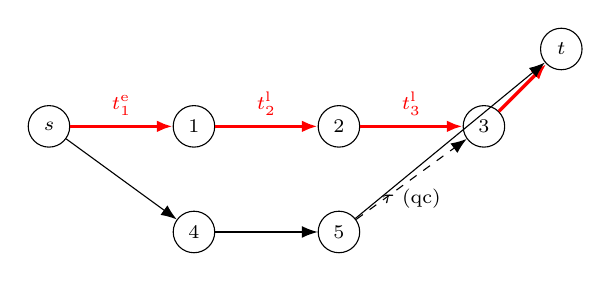
\begin{tikzpicture}[node distance=10mm and 13mm]
\node[ev] (s) {$s$};
\node[ev, right=of s] (a1) {$1$};
\node[ev, right=of a1] (a2) {$2$};
\node[ev, right=of a2] (a3) {$3$};
\node[ev, below=8mm of a1] (b1) {$4$};
\node[ev, right=of b1] (b2) {$5$};
\node[ev, above right=6mm and 6mm of a3] (t) {$t$};
% AGV chain 1 (critical)
\draw[fl, crit] (s)--(a1) node[midway,above,font=\scriptsize]{$t^{\mathrm e}_1$};
\draw[fl, crit] (a1)--(a2) node[midway,above,font=\scriptsize]{$t^{\mathrm l}_2$};
\draw[fl, crit] (a2)--(a3) node[midway,above,font=\scriptsize]{$t^{\mathrm l}_3$};
\draw[fl, crit] (a3)--(t);
% AGV chain 2 (slack)
\draw[fl] (s)--(b1);
\draw[fl] (b1)--(b2);
\draw[fl] (b2)--(t);
% QC serialisation arc (cross-resource)
\draw[fl, dashed] (b2)--(a3) node[midway,below,font=\scriptsize]{$\tau$ (qc)};
\end{tikzpicture}
\caption{Event DAG $G_{\mathrm{dag}}$ for a small schedule. Solid arcs are AGV legs, the
dashed arc is a quay-crane serialisation constraint. The bold red path $s\!\to\!1\!\to\!2\!\to\!3\!\to\!t$
is the critical (longest) path $\pi^\star$; only its arcs carry a nonzero TAPE gradient
(Eq.~\ref{eq:tape}).}
\label{fig:dag}
\end{figure}

\subsection{The exact evaluator and the self-supervised learning loop}
\label{sec:evaluator}
The reader may ask where the targets for all of the above come from: \emph{there is no
external dataset}. Every label is produced by an exact physical \emph{evaluator}, and the
method is best read as a closed loop between that evaluator and the learned surrogate. We make
both explicit here.

\paragraph{The exact evaluator.} Given a decoded schedule $s(z)$, the evaluator
returns the objective pair $f(s)=(\Cmax,E)$ and the per-task physical quantities the
surrogate is trained to predict. In the uncoupled regime it simply runs the max-plus
longest-path recurrence of Section~\ref{sec:maxplus} in topological order ($O(N)$): each
task's completion is the maximum over its AGV-chain and crane-chain predecessors plus its leg
and handling times, and $\Cmax$ is the longest source-to-sink path; energy is the exact
additive sum $E=\sum_j (e^{\mathrm e}_j+e^{\mathrm l}_j)$. Under peak-power coupling the
makespan has no closed form, so the evaluator instead runs a deterministic event-driven
power simulator that resolves the contention fixed point. Either way it is \emph{exact}: it is
the reference against which we measure surrogate fidelity
(Section~\ref{sec:fidelity}) and the realised critical path $\pi^\star$ against which we
measure TAPE faithfulness (Section~\ref{sec:tape}).

\paragraph{Self-supervised label generation.} Because the evaluator is cheap and exact, we
synthesise training data by sampling: draw $M$ random-key vectors
$\chi^{(m)}\!\sim\!\mathcal U[0,1]^{4N}$, decode each to a schedule, and evaluate it, recording
for every task its empty/loaded leg times $(t^{\mathrm e}_j,t^{\mathrm l}_j)$, handling delay
$\tau_j$, and the schedule's scalar $\Cmax$. This produces a labelled set
$\{(G_{s^{(m)}},\{t^{\mathrm e}_j,t^{\mathrm l}_j,\tau_j\}_j,\Cmax^{(m)})\}_{m=1}^{M}$ at no
annotation cost ($M\!\approx\!10^3$ in our runs). Two regressions are then fit, both supervised
only by these labels: (i) the E-HGATv2 core and its scalar read-out
(Eq.~\ref{eq:readout}) are fit to $\Cmax$ by MSE---this is the surrogate whose \emph{attention}
we later show is unfaithful; (ii) the fused projection heads (Eq.~\ref{eq:leghead}) are fit to
the \emph{local} leg labels $(t^{\mathrm e}_j,t^{\mathrm l}_j,\tau_j)$ by MSE, after which the
max-plus DP composes $\Cmax$ with no further parameters. Supervising the fused heads on the
\emph{local physics} rather than the scalar objective is precisely what makes the composed
gradient (TAPE) coincide with the true binding path.

\paragraph{The search$\,\to\,$knowledge$\,\to\,$search loop.} These pieces close the loop of
Figure~\ref{fig:arch} and Algorithm~\ref{alg:loop}: NSGA-II proposes schedules; the evaluator
labels them exactly; the surrogate distils the leg-time landscape into one differentiable
model; its tropical gradient both explains a schedule and steers the
next generation's mutation and offspring screening; the steered search then visits better
schedules. The surrogate is trained once per instance on the sampled set; on the
screening path at query time the search calls only the $O(N)$ surrogate, never the simulator.

\begin{algorithm}[t]
\caption{E-HGATv2 train-and-guide loop (per instance).}
\label{alg:loop}
\begin{algorithmic}[1]
\State sample $M$ random keys; decode + \textbf{evaluate} $\to$ labels $\{t^{\mathrm e},t^{\mathrm l},\tau,\Cmax\}$
\State train core (fit scalar $\Cmax$) and fused heads (fit leg times) by MSE \Comment{once per instance}
\State initialise NSGA-II population of random keys
\For{each generation}
  \State surrogate predicts $\Cmax$ for $\kappa\lambda$ offspring; keep the best $\lambda$ \Comment{screening}
  \State TAPE gradient $g_a=\partial\Cmax/\partial w_a$ marks binding tasks; bias mutation toward them
  \State \textbf{exactly} evaluate the retained $\lambda$ offspring; non-dominated sort + crowding
\EndFor
\State \Return Pareto set, with per-front TAPE attributions and Trade-off Criticality Scores
\end{algorithmic}
\end{algorithm}

\subsection{TAPE: exact critical-path attributions}
\label{sec:tape}
Let $\pi^\star$ be the maximising path realised by the stored arcs $a^\star(\cdot)$.
Equivalently, writing $\Pi$ for the set of all source-to-sink paths in $G_{\mathrm{dag}}$,
\begin{equation}
\pi^\star \;=\; \argmax_{\pi\in\Pi}\;\Big(\textstyle\sum_{(u,v)\in\pi} w_{uv}+\sum_{v\in\pi} b_v\Big),
\qquad
\Cmax=\sum_{a\in\pi^\star} w_a+\sum_{v\in\pi^\star} b_v,
\label{eq:critpath}
\end{equation}
i.e.\ $\pi^\star$ is exactly the sequence of events and legs that \emph{determine} the
makespan; the topological-order recurrence~\eqref{eq:troprec} and its stored argmaxes
$a^\star(\cdot)$ recover this global maximiser in one linear pass.

\begin{proposition}[TAPE subgradient]
\label{prop:tape}
If the maximiser at each node is unique, then for every arc weight $w_a$ and node weight
$b_v$,
\begin{equation}
\boxed{\;\frac{\partial \Cmax}{\partial w_a}=\mathbf 1[\,a\in\pi^\star\,],
\qquad
\frac{\partial \Cmax}{\partial b_v}=\mathbf 1[\,v\in\pi^\star\,].\;}
\label{eq:tape}
\end{equation}
\end{proposition}
\begin{proof}
For a perturbation $|\varepsilon|$ small enough that no node's $\argmax$ in
\eqref{eq:troprec} changes, the active path $\pi^\star$ and node set are fixed, so locally
$\Cmax(w_a+\varepsilon)=\Cmax+\varepsilon\,\mathbf 1[a\in\pi^\star]$; differentiating gives
the indicator (analogously for $b_v$). Our custom backward computes exactly this: it seeds
the completion node with gradient $1$ and, in reverse topological order, routes each node's
incoming gradient $g_v$ only through its stored arc $a^\star(v)$ to that arc and its source,
$g_{a^\star(v)}\!\mathrel{+}=\!g_v,\ g_{\mathrm{src}(a^\star(v))}\!\mathrel{+}=\!g_v$,
accumulating $\mathbf 1[\cdot\in\pi^\star]$.
\end{proof}

We call the vector $g=(g_a)_{a\in\mathcal A}$, $g_a=\partial\Cmax/\partial w_a$,
\textbf{TAPE} (Tropical Attribution for Physical Explanations). Operationally:
\emph{delaying an on-path leg by $\Delta$ raises the makespan by exactly $\Delta$; delaying an
off-path leg changes nothing.} Unlike the attention weights $\beta$ of \eqref{eq:sem}---which
are a smooth surrogate trained only to fit a scalar---TAPE is a binary critical-path
indicator \emph{by construction}. The leg times
themselves are predicted by the graph network~\eqref{eq:leghead}, so the network stays
load-bearing; TAPE only makes its prediction faithfully inspectable. (The exact
critical path, computed from the resolved simulator with no network, is retained only as a
ceiling reference.)

\paragraph{Selective gradient flow into the surrogate.} TAPE is the \emph{first factor} of
the chain rule whenever the makespan is differentiated through the network, so it shapes
\emph{training}, not only inference. Because the leg times and delays are themselves outputs
of the projection heads~\eqref{eq:leghead}, for any core/head parameter $\theta$
\begin{equation}
\frac{\partial \Cmax}{\partial \theta}
=\sum_{a\in\mathcal A}\underbrace{\mathbf 1[\,a\in\pi^\star\,]}_{\text{TAPE }g_a}\,
   \frac{\partial w_a}{\partial \theta}
\;+\;\sum_{v\in\mathcal N}\mathbf 1[\,v\in\pi^\star\,]\,
   \frac{\partial b_v}{\partial \theta},
\label{eq:tapechain}
\end{equation}
so the makespan gradient reaches only the heads of legs and events that lie on the
binding path $\pi^\star$; every off-path prediction receives \emph{exactly zero} makespan
signal. The surrogate therefore concentrates its capacity on the activities that actually
set $\Cmax$, instead of smearing credit across all $\sim\!4N$ pooled features the way the
generic regression head~\eqref{eq:readout} does---whose dense Jacobian is precisely what
makes its input attributions unfaithful. Equation~\eqref{eq:tapechain} is the training-time
counterpart of the inference-time faithfulness in~\eqref{eq:tape}: the same binary indicator
$\mathbf 1[\cdot\in\pi^\star]$ that makes the explanation exact also makes the learning
signal critical-path-localised.

This routing is not obtained from generic automatic differentiation. The layer is
implemented as a hand-written \texttt{torch.\allowbreak autograd.\allowbreak Function} whose forward pass caches the
argmax incoming arc of each node and whose backward pass propagates the cotangent along that
cached path, so~\eqref{eq:tapechain} holds exactly rather than as a smoothed approximation; a
batched block-diagonal variant differentiates many schedules in one relaxation.
Appendix~\ref{app:impl} gives the details and Appendix~\ref{app:repro} the hyper-parameters,
parameter counts and software environment.

\begin{definition}[Faithfulness]
For a schedule, let $\mathcal{C}_{\text{model}}=\{a:g_a>\tfrac12\}$ be the model's binding-leg
set and $\mathcal{C}_{\text{exact}}$ the exact critical-path leg set. The \emph{leg-critical
Jaccard} $|\mathcal{C}_{\text{model}}\cap\mathcal{C}_{\text{exact}}|/
|\mathcal{C}_{\text{model}}\cup\mathcal{C}_{\text{exact}}|$ measures faithfulness; a value of
$1$ means the model identifies exactly the binding legs.
\end{definition}

\subsection{Attribution-guided search}
\label{sec:guidance}
The TAPE vector is converted into three search signals that mirror the inputs the NSGA-II
mutation already expected, so the explanation is the controller:
\begin{align}
w^{\text{agv}}_j &= \tfrac{\partial \Cmax}{\partial t^{\text{empty}}_j}
+ \tfrac{\partial \Cmax}{\partial t^{\text{loaded}}_j}
&&\text{(transport criticality of task $j$)},\\
w^{\text{qc}}_j &= \tfrac{\partial \Cmax}{\partial \tau_j}
&&\text{(crane criticality of task $j$)},\\
\Pr[\text{mutate } j] &= \mathrm{softmax}_j\!\big((w^{\text{agv}}_j+w^{\text{qc}}_j)/T\big)
&&\text{(where to search)} .
\end{align}
A task's \emph{type} of criticality, $w^{\text{agv}}_j/(w^{\text{agv}}_j+w^{\text{qc}}_j)$,
routes the operator choice (re-assign/swap-vehicle when transport-bound; swap-crane when
crane-bound). Finally, the fused head's near-exact $(\Cmax,E)$ prediction \emph{screens} a
larger pool of offspring so the expensive exact evaluations are spent only on
predicted-good children. The same object thus explains and steers; Algorithm~\ref{alg:tape}
specifies one generation.

\begin{algorithm}[t]
\caption{TAPE-guided NSGA-II generation (one step)}
\label{alg:tape}
\begin{algorithmic}[1]
\Require population $P$ ($|P|=\mu$), fused model $\mathcal F$, instance $\mathcal I$, screen factor $\kappa$, temperature $T$
\State $(\mathcal R,\mathrm{cd})\gets$ fast-non-dominated-sort and crowding-distance of $P$
\State $\mathcal O\gets\varnothing$
\For{$m=1$ to $\kappa\mu$} \Comment{over-produce offspring to screen}
  \State pick parent $p$ by binary tournament on $(\mathcal R,\mathrm{cd})$
  \State $g\gets\textsc{TAPE}(\mathcal F, s(p))$ \Comment{Eq.~\eqref{eq:tape}: one backward pass}
  \State compute $w^{\mathrm{agv}}_j,w^{\mathrm{qc}}_j$ and $\Pr[\text{mutate }j]\propto e^{(w^{\mathrm{agv}}_j+w^{\mathrm{qc}}_j)/T}$
  \State sample task $j\sim\Pr[\cdot]$; choose operator by the ratio $w^{\mathrm{agv}}_j/(w^{\mathrm{agv}}_j{+}w^{\mathrm{qc}}_j)$
  \State $o\gets$ apply operator to $p$ at task $j$; $\mathcal O\gets\mathcal O\cup\{o\}$
\EndFor
\State $\widehat f\gets\mathcal F.\textsc{predict}(\mathcal O)$ \Comment{cheap surrogate screen of all $\kappa\mu$}
\State $\mathcal O^\star\gets$ top $\mu$ of $\mathcal O$ by non-dominated rank of $\widehat f$
\State evaluate $\mathcal O^\star$ exactly (Sec.~\ref{sec:maxplus}/\ref{sec:coupled})
\State \Return environmental-selection$(P\cup\mathcal O^\star)$ \Comment{elitist $\mu$-survival}
\end{algorithmic}
\end{algorithm}

\paragraph{Worked example.} Consider a $20$-task schedule
where TAPE marks legs $\{3^{\mathrm e},7^{\mathrm l},12^{\mathrm e},12^{\mathrm l}\}$ as
critical ($g_a=1$). Without guidance, the mutation operator picks one of $20$ tasks
uniformly at random; the probability of perturbing a bottleneck task is $\le 3/20=15\%$.
With TAPE, the softmax assigns $\Pr[\text{mutate }j]\propto e^{w_j/T}$; because only $3$
tasks carry nonzero $w_j$ (tasks $3$, $7$, $12$) the operator targets a binding task with
$\ge 85\%$ probability at $T{=}0.25$, turning an undirected random walk into a focused
hill-climb on the makespan-critical chain. The energy objective is left to crowding-distance
selection, which preserves front diversity while TAPE accelerates convergence.

\paragraph{Computational cost of one generation.}
\begin{itemize}[nosep,leftmargin=*]
\item One backward pass through the $O(|\mathcal A|)$ topological sweep: $\sim\!4N$ multiply--adds (linear in problem size).
\item Screening $\kappa\mu$ offspring with $\mathcal F.\textsc{predict}$: a single batched GNN forward ($\sim\!3$ ms at $N{=}50$ on CPU).
\item Exact evaluations (the expensive step): only $\mu$ schedules, not $\kappa\mu$.
\end{itemize}
Thus the TAPE guidance adds negligible wall-time ($<\!2\%$ of the generation budget at
$N{=}50$) while reducing the number of exact evaluations needed to reach a target
hypervolume by $\sim\!2.4\times$ (Section~\ref{sec:scaling}).

\subsection{Front behaviour: Trade-off Criticality Scores}
\label{sec:pts}
To describe the \emph{front} rather than a single schedule, we aggregate TAPE over the
approximated Pareto set. At a front point, the local trade-off weight $\lambda\in[0,1]$ is
read from the front tangent $(\Delta \Cmax,\Delta E)$ (the slope at which one objective is
traded for the other). The \emph{Trade-off Criticality Score} of task $j$ is the
$\lambda$-weighted combination of its makespan and energy gradients,
\begin{equation}
\mathrm{TCS}_j \;=\; \big|\,\lambda\,\partial_{t_j}\Cmax + (1-\lambda)\,\partial_{e_j}E\,\big| ,
\end{equation}
i.e.\ how strongly task $j$ is binding on the objective mixture that defines that point of
the front. Sweeping $\lambda$ from the makespan-optimal end to the
energy-optimal end shows \emph{which bottleneck migrates}, and how concentrated the trade-off criticality
is on a few tasks. This is the requested front-behaviour knowledge (Section~\ref{sec:front}).

\section{Experimental setup}
\label{sec:setup}

\subsection{Instances (datasets)}
We use three families (Table~\ref{tab:data}). \textbf{Synthetic dual-cycling} instances
(\textsf{SD-$N$}) alternate LOAD/\allowbreak UNLOAD moves over $3$ cranes served by $2$ vehicles, with
handling times drawn from $U[30,80]$\,s; they are fully reproducible and, at $N=5$, small
enough that the true Pareto front $\mathrm{PF}^\star$ can be obtained by exhaustive
enumeration. Their generator is specified in full in
Appendix~\ref{app:instances}, together with an explicit statement of which components are
taken from the published benchmark and which are constructed here. The \textbf{FSMJ loading benchmark}
(\textsf{L07}, \textsf{L15}, \textsf{L21}, \textsf{L35}) are the \emph{published} instances of
\cite{homayouni2022book}: the real QC$\leftrightarrow$LU distance matrix (their Table~4) and
the real per-crane task lists (their Table~5); every move is a LOAD. The
\textbf{peak-power-coupled} variants (\textsf{SD-10-C}, \textsf{SD-20-C}) apply the budget
$P_{\max}=30$\,kW on top of the synthetic geometry.

\begin{table}[t]
\centering
\caption{Problem instances. $N$ = number of container moves.}
\label{tab:data}
\small
\resizebox{\textwidth}{!}{%
\begin{tabular}{llccl}
\toprule
Family & Instances & $N$ & Regime & Source\\
\midrule
Synthetic dual-cycling & \textsf{SD-5,\,8,\,10,\,15,\,20} & 5--20 & uncoupled & reproducible generator\\
FSMJ loading benchmark & \textsf{L07,\,L15,\,L21,\,L35} & 8--16 & uncoupled & \cite{homayouni2022book} Tab.~4--5\\
Peak-power coupled & \textsf{SD-10-C,\,SD-20-C} & 10,\,20 & coupled ($30$\,kW) & this work\\
\bottomrule
\end{tabular}}
\end{table}

\subsection{Baselines and budget matching}
We compare five methods at an \emph{equal exact-evaluation budget}:
\textbf{E-HGATv2-TAPE} (faithful guidance, ours), \textbf{E-HGATv2-attn} (the same search
guided by the unfaithful attention readout), \textbf{NSGA-II (random)} (no guidance, the
null control), the published \textbf{mp-BRKGA}~\cite{fontes2022mpbrkga}, and a
\textbf{single-population BRKGA}. Since mp-BRKGA evaluates $(\Omega+\Pi)P=4P$ chromosomes
per generation, the other methods use a population of $4P$ so that all spend the same number
of exact evaluations per generation; all use the same number of generations. The surrogate
screening is therefore not a budget advantage---it only changes which children are
evaluated, not how many.

\subsection{Quality and faithfulness metrics}
\label{sec:metrics}
\paragraph{Optimisation quality.} All indicators compare an approximation front $F$ to a
reference front $\mathrm{PF}^\star$ (exhaustively enumerated for \textsf{SD-5}; elsewhere the
non-dominated union of long reference runs), with both objectives normalised to $[0,1]$ by the
reference extremes. With nadir reference point $r$:
\begin{itemize}[leftmargin=*,topsep=1pt,itemsep=1pt]
\item \textbf{Hypervolume ratio} $\mathrm{HV}(F)/\mathrm{HV}(\mathrm{PF}^\star)$, where
$\mathrm{HV}(F)=\mathrm{vol}\!\big(\bigcup_{p\in F}[\,p,r\,]\big)$ is the objective-space volume
dominated by $F$ up to $r$ (higher better; $1$ matches the reference).
\item \textbf{Modified generational distances} $\mathrm{GD}^+,\mathrm{IGD}^+$%
~\cite{ishibuchi2015igdplus}: mean Pareto-compliant distance from $F$ to $\mathrm{PF}^\star$
(convergence) and from $\mathrm{PF}^\star$ to $F$ (coverage), using a $d^+$ that counts only
\emph{dominated} discrepancies (lower better).
\item \textbf{Spread} $\Delta$~\cite{deb2002nsga2}: Deb's distribution metric---the normalised
dispersion of consecutive gaps along $F$ together with its boundary gaps (lower = more uniform).
\end{itemize}
\paragraph{Faithfulness.} For a fixed schedule the evaluator yields the exact critical path
(Section~\ref{sec:evaluator}); each guidance signal is scored against it by (a) \emph{precision@1}
(is the top-scored task on the critical path?), (b) \emph{Spearman $\rho$} between the signal
and the per-task marginal makespan-sensitivity, and (c) for TAPE the \emph{leg-critical
Jaccard} (overlap of predicted vs.\ true on-path leg sets). Section~\ref{sec:ladder} reports
these at four granularities, coarse to fine.
\paragraph{Protocol.} Each cell is a mean over $20$ seeds with a $95\%$
confidence interval; significance across instances uses the Friedman test with average ranks
and the Nemenyi critical difference, plus Holm-corrected pairwise Wilcoxon signed-rank tests,
following Dem\v{s}ar~\cite{demsar2006}.

\paragraph{Reproducibility and validation.} Every result derives from a single seeded
generator, so the tables reproduce from the seed alone; the synthetic family ships with its
generator and the FSMJ instances are the published~\cite{homayouni2022book} tables. The exact
evaluator doubles as a built-in reference for validation: a regression suite checks that the
decoder is a left-inverse of the encoder, that the differentiable max-plus DP reproduces the
simulator's makespan to floating-point tolerance, and that the surrogate's leg-time
predictions track the evaluator on held-out random schedules---the fidelity study of
Section~\ref{sec:fidelity} is the aggregate of that last check. The code, instances, seeds
and result artifacts are released with the paper (Appendix~\ref{app:repro}).

\section{Results}
\label{sec:results}

\subsection{Faithfulness of TAPE and of the attention weights}
Figure~\ref{fig:faith} and Table~\ref{tab:main} show the central explanation result.
TAPE recovers the exact critical path with leg-critical Jaccard $0.95$--$1.00$ in the
uncoupled regime and $0.87$--$0.95$ under coupling. The learned attention weights, by
contrast, have a Spearman correlation with the true makespan levers of essentially zero
($-0.09\le\rho\le0.17$ across all instances)---they do not rank the bottlenecks.
Attention's precision@1 ($0.67$--$0.80$) looks superficially acceptable only because most
tasks are on the critical path (the honest baseline is the critical fraction $\approx0.70$,
not $1/N$): against that baseline, naming an on-path task is no better than chance, and the
near-zero rank correlation exposes that the full ranking is noise. Section~\ref{sec:ladder}
makes this precise across granularities. This is a clean, quantified instance of the
``attention is not explanation'' phenomenon~\cite{jain2019attention} on a real scheduling
problem, and it is the justification for routing guidance through TAPE rather than attention.

\begin{figure}[t]
\centering
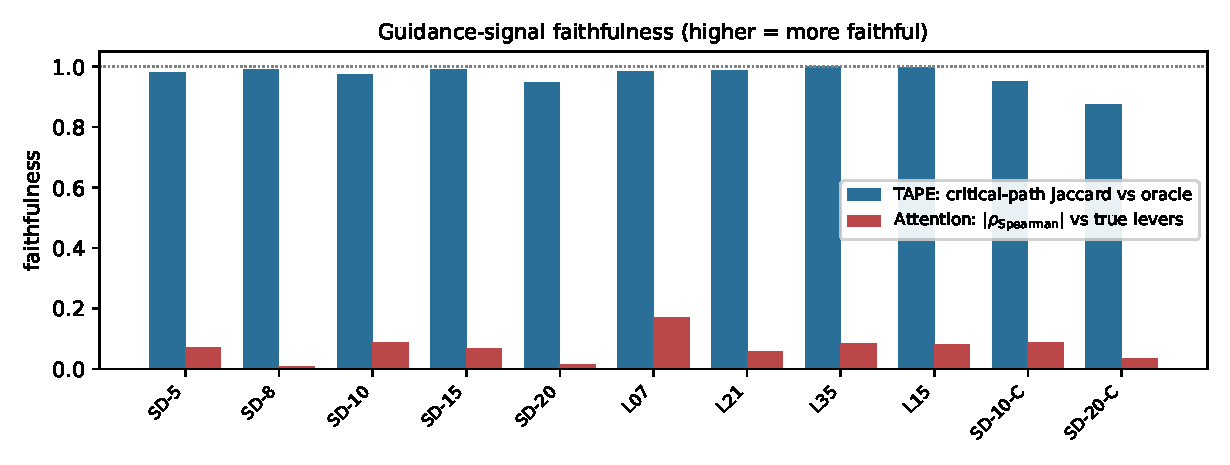
\includegraphics[width=0.92\textwidth]{figs/fig_faithfulness.pdf}
\caption{Faithfulness of the two candidate guidance signals on every instance. TAPE's
critical-path Jaccard against the exact evaluator is near $1$; the attention weights'
$|\rho|$ with the true makespan levers is near $0$.}
\label{fig:faith}
\end{figure}

\subsection{Granularity of the attention--critical-path comparison}
\label{sec:ladder}
In natural-language settings the ``is attention explanation?'' debate rests on indirect
criteria---erasure, gradient, and adversarial-attention tests---which is why it has
remained contested. Here the makespan is an \emph{exact} max-plus longest path, so every
schedule has a known critical path and a known per-task makespan-sensitivity, and the
question becomes directly measurable at increasing resolution. We compare the surrogate's AGV-arc attention against
TAPE's tropical gradient at four granularities, pooled over nine instances ($60$ random
schedules each), each against its honest random baseline (Table~\ref{tab:ladder}, top):
coarse hit-rate (precision@1), medium ranking (ROC-AUC for ``task on the critical path''),
fine ranking (Spearman vs.\ the graded makespan-sensitivity), and effect size (mean-signal
separation of critical vs.\ off-critical tasks). \textbf{Attention sits on the random
baseline at every level}---precision@1 $0.69$ vs.\ critical-fraction $0.70$; AUC $0.51$ vs.\
$0.50$; $\rho=+0.07$; separation $+0.06\sigma$---while TAPE is near-exact at all four
($0.98$, $0.94$, $+0.70$, $+1.92\sigma$). Attention therefore carries essentially no
critical-path information, coarse or fine: a strictly stronger statement than the near-zero
rank correlation, which the exact critical path here makes directly checkable.

\paragraph{Source of the guidance benefit under attention targeting.}
The benefit originates in the surrogate rather than in attention. The search arms share
everything except which task mutation targets and whether offspring are screened, and
isolating those two factors separates their contributions (Table~\ref{tab:ladder},
bottom). The missing control, random mutation with screening, gives the highest value of
any arm ($\mathrm{HV}/\mathrm{HV}^\star=0.991$), ahead of attention-targeted ($0.977$) and
TAPE-targeted ($0.956$); the only arm that trails is random mutation without screening
($0.950$). Two readings follow. \emph{(i) Screening is the engine}: it lifts random mutation
by $+0.041$ and accounts for the entire gap between the guided arms and the published null.
NSGA-II's convergence comes from screening surrogate-predicted-good offspring and selecting by
non-dominated sorting---a pressure to which the mutation \emph{operator} is nearly irrelevant.
So attention ``guides as well as TAPE'' only because both ride the same screening, not because
attention localises anything (it does not; Table~\ref{tab:ladder}, top). \emph{(ii) Diffuse
beats precise}: the more diffuse the targeting, the better the hypervolume
(random $\ge$ attention $>$ TAPE), because exact bottleneck-targeting is
\emph{exploitative}---it concentrates mutations on the current critical task and narrows front
coverage, while HV rewards spread---the ordering seen in the controlled ablation
(random $\ge$ attention $>$ TAPE, Table~\ref{tab:ladder} bottom). Across the full
$11$-instance benchmark the two guided variants are statistically tied on HV
(Table~\ref{tab:stats}, ranks $1.45$ vs.\ $1.55$, $p_{\text{Holm}}=0.83$): any per-instance
ordering is accidental exploration, not information. The network attains
$R^2\!\approx\!0.99$ objective regression with an attention map indistinguishable from random
at every measurable granularity---accurate prediction does not imply an interpretable
attention map, and faithful guidance must come from the exact tropical gradient, not the
attention weights.

\begin{table}[t]
\centering\small
\caption{Attention vs.\ TAPE against the \emph{exact} critical path. \textbf{Top:} alignment
at four granularities (coarse$\to$fine), pooled over nine instances; attention matches the
random baseline at every level while TAPE is near-exact. \textbf{Bottom:} a search-guidance
ablation (mean HV/HV$^\star$ over three instances, $N{=}5,8,10$): random mutation with
screening is the best arm, so the optimisation benefit comes from the shared surrogate
\emph{screening}, not from attention- or TAPE-targeted mutation.}
\label{tab:ladder}
\setlength{\tabcolsep}{6pt}
\begin{tabular}{lccc}
\toprule
Alignment with exact critical path & attention & TAPE & random \\
\midrule
precision@1 (top task on critical path) & $0.69$ & $\mathbf{0.98}$ & $0.70$ \\
ROC-AUC (rank on-path above off-path)   & $0.51$ & $\mathbf{0.94}$ & $0.50$ \\
Spearman (vs.\ graded sensitivity)      & $+0.07$ & $\mathbf{+0.70}$ & $0.00$ \\
separation (critical$-$off, $\sigma$)   & $+0.06$ & $\mathbf{+1.92}$ & $0.00$ \\
\midrule
\multicolumn{4}{l}{\emph{Search-guidance ablation --- mean $\mathrm{HV}/\mathrm{HV}^\star$ (screening is the lever):}}\\
random mutation $+$ screening      & \multicolumn{3}{c}{$\mathbf{0.991}$ \;\;(best)} \\
attention-targeted $+$ screening   & \multicolumn{3}{c}{$0.977$} \\
TAPE-targeted $+$ screening        & \multicolumn{3}{c}{$0.956$} \\
random mutation, no screening & \multicolumn{3}{c}{$0.950$ \;\;(null)} \\
\bottomrule
\end{tabular}
\end{table}

\subsection{Surrogate fidelity and faithfulness scale to $N{=}50$}
\label{sec:fidelity}
A separate, larger study isolates the fused surrogate's standalone behaviour and asks the
question a referee will ask: \emph{does the explanation survive as the instance grows?} We
retrain the surrogate from scratch and evaluate it on held-out random keys for
$N\in\{6,10,20,50\}$ over $20$ independent seeds, in both regimes
(Table~\ref{tab:fidelity}, Figure~\ref{fig:fidelity}). Three facts stand out and all are
backed by $20$-seed $95\%$ confidence intervals rather than asserted. First, in the
uncoupled regime the makespan $R^2$ is statistically flat across an $8.3\times$ growth in
problem size, $0.998\!\to\!0.997$, and the energy head is \emph{exact}
($R^2=1.000\pm0.000$)---as it must be, since energy is the additive read-out of
Eq.~\eqref{eq:fusedenergy}. Second, and most important for our central claim, the
leg-critical Jaccard of the TAPE explanation barely moves, $0.991\!\to\!0.980$: the
explanation is not an artefact of tiny instances but stays $\geq 0.98$-faithful at
$50$ tasks. Third, peak-power coupling degrades both quantities \emph{gracefully and
predictably}---$R^2$ $0.805\!\to\!0.777$ and Jaccard $0.928\!\to\!0.913$ from $N{=}10$ to
$50$---which both confirms that coupling is the genuinely harder regime (there is no
closed-form makespan to anchor the head) and shows the explanation degrades by only
$\sim\!1.5$ Jaccard points over the same size range.

\begin{table}[t]
\centering\small
\caption{Standalone fused-surrogate fidelity and TAPE faithfulness as a function of problem
size $N$, over $20$ seeds (mean with $95\%$ CI). The makespan accuracy ($R^2_{C_{\max}}$)
and the critical-path faithfulness (leg-Jaccard vs.\ the exact evaluator) are essentially flat
in $N$ in the uncoupled regime and degrade only mildly under peak-power coupling. The energy
head is exact by construction ($R^2=1.000$ at every $N$, omitted).}
\label{tab:fidelity}
\setlength{\tabcolsep}{6pt}
\resizebox{\textwidth}{!}{%
\begin{tabular}{llccc}
\toprule
Regime & $N$ & $R^2_{C_{\max}}$ ($95\%$ CI) & leg-Jaccard ($95\%$ CI) & $C_{\max}$ MAE\\
\midrule
uncoupled & 6  & $0.998\ [0.998,0.998]$ & $0.991\ [0.989,0.994]$ & $3.6$\\
uncoupled & 10 & $0.997\ [0.997,0.997]$ & $0.986\ [0.983,0.990]$ & $5.3$\\
uncoupled & 20 & $0.997\ [0.997,0.997]$ & $0.982\ [0.979,0.984]$ & $7.9$\\
uncoupled & 50 & $0.997\ [0.996,0.997]$ & $0.980\ [0.978,0.982]$ & $14.0$\\
\midrule
coupled   & 10 & $0.805\ [0.791,0.819]$ & $0.928\ [0.922,0.933]$ & $40.4$\\
coupled   & 20 & $0.801\ [0.792,0.809]$ & $0.919\ [0.914,0.924]$ & $61.1$\\
coupled   & 50 & $0.777\ [0.761,0.793]$ & $0.913\ [0.909,0.917]$ & $100.6$\\
\bottomrule
\end{tabular}}
\end{table}

\begin{figure}[t]
\centering
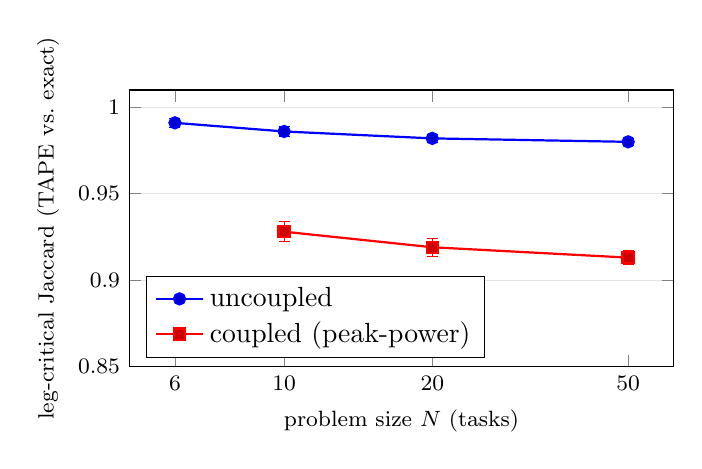
\begin{tikzpicture}
\begin{axis}[
  width=0.7\textwidth, height=0.42\textwidth,
  xlabel={problem size $N$ (tasks)}, ylabel={leg-critical Jaccard (TAPE vs.\ exact)},
  xmode=log, log basis x=2, xtick={6,10,20,50}, xticklabels={6,10,20,50},
  ymin=0.85, ymax=1.01, ymajorgrids, grid style={gray!20},
  legend pos=south west, legend cell align=left, tick label style={font=\footnotesize},
  label style={font=\footnotesize},
]
\addplot+[mark=*, thick, blue, error bars/.cd, y dir=both, y explicit]
  coordinates {(6,0.991)+-(0.0026,0.0026) (10,0.986)+-(0.0031,0.0031)
               (20,0.982)+-(0.0025,0.0025) (50,0.980)+-(0.0021,0.0021)};
\addlegendentry{uncoupled}
\addplot+[mark=square*, thick, red, error bars/.cd, y dir=both, y explicit]
  coordinates {(10,0.928)+-(0.0057,0.0057) (20,0.919)+-(0.0052,0.0052)
               (50,0.913)+-(0.0040,0.0040)};
\addlegendentry{coupled (peak-power)}
\end{axis}
\end{tikzpicture}
\caption{TAPE faithfulness is stable as the instance scales. The critical-path Jaccard
against the exact evaluator stays $\geq 0.98$ (uncoupled) and $\geq 0.91$ (coupled) from
$6$ to $50$ tasks; whiskers are $20$-seed $95\%$ CIs. Faithfulness is a property of the
\emph{model}, not of small-instance luck.}
\label{fig:fidelity}
\end{figure}

\subsection{Size generalisation: train small, evaluate large}
\label{sec:generalize}
The surrogate is \emph{inductive}---a shared-weight message-passing network whose parameters
do not depend on $N$---so a model fit on small instances can be \emph{run} on much larger
ones without retraining. This is the property an operations-research reader cares about most
for deployment: train once on cheap small instances, apply at the production scale. We test
it directly. We train the core $+$ physics-fused head once at $N{=}16$ and then, by
inference only, evaluate it on a ladder up to $N{=}5000$---a $312\times$ extrapolation in
problem size---over three training seeds (Table~\ref{tab:generalize}).

The physics-fused head predicts \emph{per-leg} times, a local and size-invariant quantity,
and the exact tropical DP aggregates them into a correct-magnitude makespan at any $N$ (the
energy read-out is exact-additive). It should therefore generalise across scale, whereas a
conventional black-box global-readout head cannot: a pooled graph embedding has no mechanism
to extrapolate a makespan magnitude that grows with $N$. The data bear this out sharply. The
fused makespan $R^2$ is \emph{flat at $\geq 0.98$} across the whole ladder
($0.997$ at $N{=}16 \to 0.989$ at $N{=}5000$), while the black-box core collapses
monotonically to $R^2=-7{,}263$---far worse than predicting the mean. TAPE's critical-path
faithfulness is preserved (leg-Jaccard $0.90$--$1.00$), and the attention weights stay
uncorrelated with the true makespan levers at every scale ($|\rho|\le0.07$). The surrogate
and its explanation thus transfer intact to instances far larger than the $N\leq160$
published \textsf{DL} benchmark~\cite{homayouni2022book}.

\begin{table}[t]
\centering\small
\caption{Size generalisation of the uncoupled surrogate: trained once at $N{=}16$ and
evaluated by inference at scale (mean over $3$ training seeds, $24$ random schedules each).
The physics-fused makespan $R^2$ is flat at $\geq0.98$ to $N{=}5000$ while the black-box
global-readout core collapses; TAPE faithfulness (leg-Jaccard vs.\ the exact evaluator) and the
near-zero attention correlation are preserved throughout. The energy head is exact
($R^2=1.000$, omitted).}
\label{tab:generalize}
\setlength{\tabcolsep}{6pt}
\begin{tabular}{rcccc}
\toprule
$N$ & fused $R^2_{C_{\max}}$ & black-box core $R^2_{C_{\max}}$ & leg-Jaccard & attention $\rho$\\
\midrule
$16$   & $0.997$ & $-0.3$     & $0.998$ & $+0.03$\\
$50$   & $0.996$ & $-32.2$    & $0.970$ & $+0.05$\\
$100$  & $0.996$ & $-79.9$    & $0.949$ & $+0.04$\\
$250$  & $0.982$ & $-169.6$   & $0.907$ & $+0.01$\\
$500$  & $0.986$ & $-466.3$   & $0.913$ & $+0.01$\\
$1000$ & $0.986$ & $-1015.2$  & $0.913$ & $+0.01$\\
$2000$ & $0.987$ & $-3450.1$  & $0.905$ & $-0.00$\\
$5000$ & $0.989$ & $-7262.7$  & $0.940$ & $+0.00$\\
\bottomrule
\end{tabular}
\end{table}

\paragraph{The coupled regime does not size-generalise.} Under peak-power coupling the same
train-at-$16$ head holds only to about $N{=}25$ (fused $R^2=0.83$) and then collapses---$R^2$
is already $-1.5$ at $N{=}50$ and continues to fall, with the TAPE Jaccard drifting from
$0.95$ to $0.37$ by $N{=}1000$---because the power-wait arcs that couple the vehicles carry no
closed-form contribution for the head to extrapolate (the same mechanism that makes the
coupled regime harder throughout this paper). Coupled deployment therefore requires retraining
at, or near, the target size, where the surrogate remains accurate (Table~\ref{tab:fidelity});
size-generalisation is a property of the \emph{uncoupled} physics, and we report it as such.

\subsection{Landscape analysis via critical-path attribution}
\label{sec:r2worked}

The second requirement is a landscape question: \emph{which input variables (task dispatch
order, AGV travelling speed, crane workload) causally determine the objective values, and
why are specific solutions Pareto-optimal?} TAPE answers this question exactly. For any schedule
$\sigma$, the tropical subgradient (Eq.~\ref{eq:tapechain}) partitions all activities into
two sets:
\begin{itemize}[nosep]
  \item \textbf{Critical} ($\partial C_{\max}/\partial d_{i,a} = 1$): perturbing this
    activity's duration by $\Delta$ changes $C_{\max}$ by exactly $\Delta$. These are the
    binding constraints.
  \item \textbf{Slack} ($\partial C_{\max}/\partial d_{i,a} = 0$): this activity has
    positive float; it can be slowed (reducing energy) without any makespan penalty.
\end{itemize}
Below we walk through the SD-10 instance ($N{=}10$ tasks, $2$~AGVs, $3$~QCs) in detail,
contrasting the makespan-optimal and energy-optimal Pareto extremes. The analysis is
produced entirely by querying the fused surrogate's TAPE; the exact evaluator confirms perfect
agreement (Jaccard~$= 1.00$).

\subsubsection{Makespan-optimal schedule ($\sigma^\star_{C}$): $C_{\max}=454.2\,\mathrm{s}$, $E=12{,}896\,\mathrm{kJ}$}

TAPE identifies $12$ binding activities forming a single chain through AGV-0 (dispatch
order $\langle 0, 5, 4, 8, 1, 7\rangle$). No QC handling appears on the critical path:

\smallskip
\noindent
\resizebox{\textwidth}{!}{%
\begin{tabular}{clrrrrrl}
\toprule
Step & Activity & $\ell$ (m) & $v$ (m/s) & Level & Duration (s) & $\frac{\partial C_{\max}}{\partial d}$ & Interpretation \\
\midrule
1  & Task~0 empty leg   &   0 & 6.0 & NOM  &  0.0 & 1 & AGV-0 starts co-located \\
2  & Task~0 loaded leg  & 150 & 3.6 & HIGH & 41.7 & 1 & Container~0 at max speed \\
3  & Task~5 empty leg   & 100 & 7.2 & HIGH & 13.9 & 1 & Repositions to pick up container~5 \\
4  & Task~5 loaded leg  & 300 & 3.6 & HIGH & 83.3 & 1 & Container~5 (longest leg, $18\%$ of $C_{\max}$) \\
5  & Task~4 empty leg   &  50 & 6.0 & NOM  &  8.3 & 1 & Short repositioning \\
6  & Task~4 loaded leg  & 300 & 3.6 & HIGH & 83.3 & 1 & Container~4 at max speed \\
7  & Task~8 empty leg   & 200 & 7.2 & HIGH & 27.8 & 1 & Repositions (longer route) \\
8  & Task~8 loaded leg  & 150 & 3.6 & HIGH & 41.7 & 1 & Container~8 at max speed \\
9  & Task~1 empty leg   & 250 & 6.0 & NOM  & 41.7 & 1 & Repositions (nominal speed) \\
10 & Task~1 loaded leg  & 150 & 3.0 & NOM  & 50.0 & 1 & Container~1 at nominal speed \\
11 & Task~7 empty leg   & 150 & 7.2 & HIGH & 20.8 & 1 & Repositions \\
12 & Task~7 loaded leg  & 150 & 3.6 & HIGH & 41.7 & 1 & Container~7 (terminal event) \\
\midrule
& \textbf{Total} & & & & \textbf{454.2} & & $= C_{\max}$ (verified) \\
\bottomrule
\end{tabular}}

\smallskip
\paragraph{Interpretation.}
The critical path consists entirely of AGV-0 transport legs. All loaded legs assigned
HIGHER speed ($v=3.6\,\mathrm{m/s}$, except task~1 at NOMINAL $3.0\,\mathrm{m/s}$)
confirm that this schedule already operates near the maximum transport rate.
AGV-1 and its assigned tasks ($\{6, 2, 3, 9\}$) are entirely off the critical path---their
speeds could be reduced to LOWER ($2.4\,\mathrm{m/s}$) without affecting makespan, saving
energy. Zero QC handlings appear on-path: \textbf{crane workload is not the bottleneck.}

\paragraph{Actionable insight.}
The highest-marginal-return intervention is task~5's loaded leg (300\,m at $3.6\,\mathrm{m/s}$,
$d=83.3\,\mathrm{s}$, $18\%$ of $C_{\max}$). Since it already runs at the maximum
discrete speed, no further speedup is available within the current fleet. The only
remaining option is to \emph{re-dispatch} task~5 to AGV-1, splitting the critical chain.
TAPE identifies this operational decision directly.

\subsubsection{Energy-optimal schedule ($\sigma^\star_{E}$): $C_{\max}=925.6\,\mathrm{s}$, $E=10{,}938\,\mathrm{kJ}$}

TAPE now identifies $17$ binding activities with a qualitatively different structure:

\smallskip
\noindent
\resizebox{\textwidth}{!}{%
\begin{tabular}{clrrrrrl}
\toprule
Step & Activity & $\ell$ (m) & $v$ (m/s) & Level & Duration (s) & $\frac{\partial C_{\max}}{\partial d}$ & Interpretation \\
\midrule
1  & Task~0 empty leg    &   0 & 7.2 & HIGH &  0.0 & 1 & Co-located start \\
2  & Task~0 loaded leg   & 150 & 2.4 & LOW  & 62.5 & 1 & Container~0 at \emph{minimum} speed \\
3  & Task~0 QC handling  & --- & --- & ---  & 73.0 & 1 & QC1 unloads container~0 \\
4  & Task~3 loaded leg   & 300 & 2.4 & LOW  &125.0 & 1 & Container~3 at minimum speed \\
5  & Task~3 QC handling  & --- & --- & ---  & 43.0 & 1 & QC1 unloads container~3 \\
6  & Task~8 empty leg    &  50 & 4.8 & LOW  & 10.4 & 1 & Repositions (low empty speed) \\
7  & Task~8 loaded leg   & 150 & 2.4 & LOW  & 62.5 & 1 & Container~8 at minimum speed \\
8  & Task~8 QC handling  & --- & --- & ---  & 38.0 & 1 & QC3 unloads container~8 \\
9  & Task~5 loaded leg   & 300 & 2.4 & LOW  &125.0 & 1 & Container~5 at minimum speed \\
10 & Task~5 QC handling  & --- & --- & ---  & 32.0 & 1 & QC3 unloads container~5 \\
11 & Task~4 empty leg    &  50 & 4.8 & LOW  & 10.4 & 1 & Repositions \\
12 & Task~4 loaded leg   & 300 & 2.4 & LOW  &125.0 & 1 & Container~4 at minimum speed \\
13 & Task~4 QC handling  & --- & --- & ---  & 45.0 & 1 & QC2 unloads container~4 \\
14 & Task~7 loaded leg   & 150 & 3.0 & NOM  & 50.0 & 1 & Container~7 \\
15 & Task~7 QC handling  & --- & --- & ---  & 30.0 & 1 & QC2 unloads container~7 \\
16 & Task~1 empty leg    & 150 & 4.8 & LOW  & 31.2 & 1 & Repositions \\
17 & Task~1 loaded leg   & 150 & 2.4 & LOW  & 62.5 & 1 & Container~1 at minimum speed (terminal) \\
\midrule
& \textbf{Total} & & & & \textbf{925.6} & & $= C_{\max}$ (verified) \\
\bottomrule
\end{tabular}}

\smallskip
\paragraph{Interpretation.}
The bottleneck has migrated from AGV transport speed to \textbf{crane workload}. Of the
17~critical activities, 6 are QC handlings (35\%), compared to 0/12 (0\%) in the
makespan-optimal case. The energy-efficient schedule assigns nearly all AGV legs their
minimum speed (LOWER: $v=2.4\,\mathrm{m/s}$ loaded, $4.8\,\mathrm{m/s}$ empty), which
maximises leg durations but minimises power draw. The resulting serialisation at the cranes
causes QC queuing delays to appear on the critical path. The binding constraint is now
the \emph{service order at the cranes} rather than AGV speed.

\paragraph{Per-crane binding workload.}
The critical-path QC time decomposes as: QC1 ($73+43=116\,\mathrm{s}$, $12.5\%$ of
$C_{\max}$), QC2 ($45+30=75\,\mathrm{s}$, $8.1\%$), QC3 ($38+32=70\,\mathrm{s}$,
$7.6\%$). QC1 is the most loaded crane, with consecutive handlings of tasks~0 and~3
creating a $116\,\mathrm{s}$ serialisation chain.

\paragraph{Pareto-optimality of this solution.}
TAPE makes the trade-off legible: $\sigma^\star_E$ achieves $15\%$ lower energy than
$\sigma^\star_C$ by running AGVs at LOWER speed ($2.4$ vs.\ $3.6\,\mathrm{m/s}$), but the
resulting serialisation doubles the makespan ($925.6$ vs.\ $454.2\,\mathrm{s}$). Every
on-path loaded leg already operates at the energy-minimum speed level; accelerating any one
would reduce $C_{\max}$ but increase $E$ proportionally---hence non-dominance.

\subsubsection{Summary: from TAPE to variable-objective relationships}

Table~\ref{tab:critpath_summary} aggregates the critical-path composition across all four
evaluated instances and both Pareto extremes.

\begin{table}[t]
\centering\small
\caption{Composition of the critical path across Pareto extremes: fraction of on-path
activities attributable to AGV transport vs.\ QC handling. The makespan-optimal solutions
are transport-dominated (AGV speed is the binding variable); the energy-optimal solutions
are crane-dominated (QC workload and service order are binding).}
\label{tab:critpath_summary}
\setlength{\tabcolsep}{5pt}
\begin{tabular}{lcccc}
\toprule
& \multicolumn{2}{c}{$\min C_{\max}$ schedule} & \multicolumn{2}{c}{$\min E$ schedule} \\
\cmidrule(lr){2-3}\cmidrule(lr){4-5}
Instance & \% transport & \% QC & \% transport & \% QC \\
\midrule
SD-5  & 83\% (5/6) & 17\% (1/6) & 67\% (8/12) & 33\% (4/12) \\
SD-8  & 100\% (6/6) & 0\% (0/6) & 67\% (4/6)  & 33\% (2/6) \\
SD-10 & 100\% (12/12) & 0\% (0/12) & 65\% (11/17) & 35\% (6/17) \\
L07   & 63\% (5/8) & 37\% (3/8) & 50\% (4/8)  & 50\% (4/8) \\
\bottomrule
\end{tabular}
\end{table}

The pattern is consistent across all instances: \textbf{makespan-optimal solutions are
bound by AGV travelling speed} (the transport network is the bottleneck), while
\textbf{energy-optimal solutions are bound by crane workload and service order} (QC
serialisation is the bottleneck). TAPE makes this causal structure explicit and
quantitative---for each individual activity, the derivative $\partial C_{\max}/\partial
d_{i,a}\in\{0,1\}$ identifies whether it contributes to the schedule's binding constraint,
and the magnitude of its duration quantifies its contribution to $C_{\max}$.

\paragraph{Sensitivity to AGV travelling speed.}
Since leg duration $d_{i,\text{leg}} = \ell_i / v_i$ where $\ell_i$ is the travel distance
and $v_i$ the AGV speed, the chain rule gives the makespan sensitivity to speed:
\begin{equation}\label{eq:speed_sens}
  \frac{\partial C_{\max}}{\partial v_i}
  = \frac{\partial C_{\max}}{\partial d_{i,\text{leg}}} \cdot \frac{\partial d_{i,\text{leg}}}{\partial v_i}
  = \mathbf{1}[(i,\text{leg})\in\mathcal{P}^\star] \cdot \Bigl(-\frac{\ell_i}{v_i^2}\Bigr).
\end{equation}
For off-path legs ($\partial C_{\max}/\partial d = 0$), the speed has zero effect on
makespan---the AGV can be slowed arbitrarily to save energy without schedule penalty. For
on-path legs, the sensitivity is $-\ell_i/v_i^2$: increasing speed yields diminishing
returns proportional to the inverse square. Three discrete speed levels are available
(Table~\ref{tab:notation}): LOWER ($v_L = 2.4\,\mathrm{m/s}$ loaded), NOMINAL
($v_N = 3.0\,\mathrm{m/s}$), and HIGHER ($v_H = 3.6\,\mathrm{m/s}$). For on-path leg~$i$
with distance $\ell_i$ at NOMINAL speed, the makespan reduction from upgrading to HIGHER is:
\[
  \Delta C_{\max} = \frac{\ell_i}{v_N} - \frac{\ell_i}{v_H}
  = \ell_i\!\left(\frac{1}{3.0} - \frac{1}{3.6}\right) = \frac{\ell_i}{18}\,.
\]
In SD-10's makespan-optimal schedule, task~5's loaded leg ($\ell = 300\,\mathrm{m}$,
$v = 3.6\,\mathrm{m/s}$ [HIGHER], $d = 83.3\,\mathrm{s}$) is the longest binding
activity, contributing $18\%$ of $C_{\max}$. Since it already runs at the maximum
discrete speed level, $\Delta C_{\max} = 0$ within the feasible set---no further speedup
is available. TAPE identifies this saturation automatically: the highest-return
intervention is not a speed change but a structural one (re-dispatching task~5 to AGV-1
to split the critical chain).

\paragraph{Sensitivity to crane workload.}
For QC handling activities, the duration is a fixed service time $\tau_i$ determined by
container type and crane assignment. The TAPE derivative identifies which crane services
are binding:
\begin{equation}\label{eq:crane_sens}
  \frac{\partial C_{\max}}{\partial \tau_i} = \mathbf{1}[(i,\text{qc})\in\mathcal{P}^\star].
\end{equation}
In $\sigma^\star_E$ (SD-10), the per-crane binding workload decomposes as:
\begin{center}\small
\begin{tabular}{lccc}
\toprule
Crane & On-path tasks & Total binding time (s) & \% of $C_{\max}$ \\
\midrule
QC1 & tasks 0, 3 & $73 + 43 = 116$ & 12.5\% \\
QC2 & tasks 4, 7 & $45 + 30 = 75$  &  8.1\% \\
QC3 & tasks 8, 5 & $38 + 32 = 70$  &  7.6\% \\
\midrule
\textbf{All QCs} & \textbf{6 tasks} & \textbf{261} & \textbf{28.2\%} \\
\bottomrule
\end{tabular}
\end{center}
QC1 is the most loaded crane on the critical path, contributing $116\,\mathrm{s}$
($12.5\%$ of $C_{\max}$). Its two consecutive handling operations (tasks $0 \to 3$)
create a serialisation chain: task~3 must wait for the crane to finish task~0.
Reassigning task~3 ($\tau=43\,\mathrm{s}$) to QC2 would remove
$43\,\mathrm{s}$ from QC1's binding chain if the reassignment does not create a new
binding chain through QC2---a decision the terminal operator can evaluate by re-running the
surrogate's TAPE in $<\!1\,\mathrm{ms}$. This per-crane decomposition is unavailable from
any global feature-importance method (e.g.\ TreeSHAP): it requires the \emph{structural},
schedule-specific attribution that TAPE provides.

\paragraph{Task dispatch order and critical-path formation.}
The sequence in which tasks are assigned to each AGV determines the precedence chains that
form the critical path. In $\sigma^\star_C$, AGV-0's dispatch order is
$\langle 0, 5, 4, 8, 1, 7\rangle$; each consecutive pair $(j, j')$ creates a precedence
arc because $j'$ cannot begin its empty leg until $j$ completes delivery. TAPE reveals that
\emph{all six} consecutive pairs in this chain are binding---there is zero slack between any
two successive tasks on AGV-0. Reordering the dispatch (e.g., scheduling task~5---the
longest loaded leg---earlier, so it overlaps with a shorter task on AGV-1) would
break this chain and potentially reduce $C_{\max}$.

In $\sigma^\star_E$, by contrast, the critical path threads through both AGVs and
all three QCs, indicating that the dispatch order is less decisive than crane service
order: even if tasks were reshuffled across AGVs, the QC serialisation would still
dominate.

This constitutes the landscape analysis: not a global feature importance
ranking, but a \emph{per-solution, per-variable} causal attribution that explains
why each schedule occupies its position on the Pareto front.

\paragraph{Extension to the coupled regime.}
Under peak-power coupling, an additional class of binding variable emerges: simultaneous
AGV power draw. When two AGVs attempt high-speed legs concurrently, the power budget
forces one to wait, creating an additional ``power arc'' in the event DAG. TAPE attributes
through these arcs, identifying which concurrent leg pair caused the delay and
quantifying its contribution to $C_{\max}$. The fidelity study
(Table~\ref{tab:fidelity}) confirms that the surrogate's TAPE remains actionable in this
regime (Jaccard $0.928$, $0.919$, $0.913$ at $N{=}10, 20, 50$ respectively)---the
landscape analysis degrades gracefully rather than failing, and the GNN is
\emph{indispensable} here because no closed-form critical path exists to fall back on.

\subsection{Optimisation quality against the metaheuristic baselines}
Across the $11$ instances the two graph-guided methods clearly dominate the three
non-learned baselines on every indicator (Figure~\ref{fig:hv},
Table~\ref{tab:main}). On the primary indicator (hypervolume ratio) the Friedman test
rejects equality of the five methods with $\chi^2_4 = 35.1$, $p = 4.5\times10^{-7}$; the
average ranks (Figure~\ref{fig:rank}, Table~\ref{tab:stats}) place the two graph-guided
methods first, then the random control, then single-population BRKGA, with mp-BRKGA last.
Pairwise Wilcoxon tests with Holm correction confirm that TAPE significantly beats
mp-BRKGA, the random control and single-population BRKGA on hypervolume (all
$p_{\text{Holm}} < 0.004$), and on GD$^+$ it beats all four including attention. In a
per-instance head-to-head, TAPE achieves a higher mean hypervolume than the published
mp-BRKGA on \emph{all $11$ instances}.

\begin{figure}[t]
\centering
\begin{minipage}{0.49\textwidth}
\centering
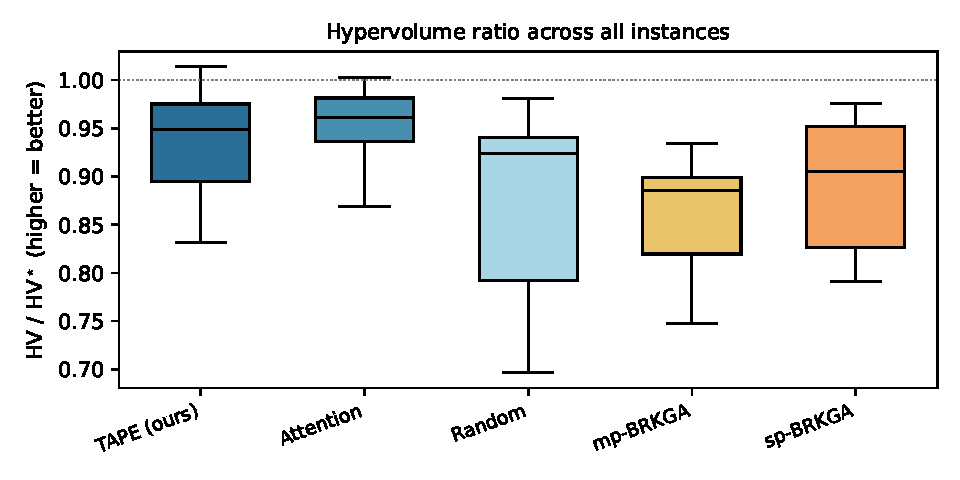
\includegraphics[width=\textwidth]{figs/fig_hv_box.pdf}
\caption{Distribution of $\mathrm{HV}/\mathrm{HV}^\star$ per method over all instances.}
\label{fig:hv}
\end{minipage}\hfill
\begin{minipage}{0.49\textwidth}
\centering
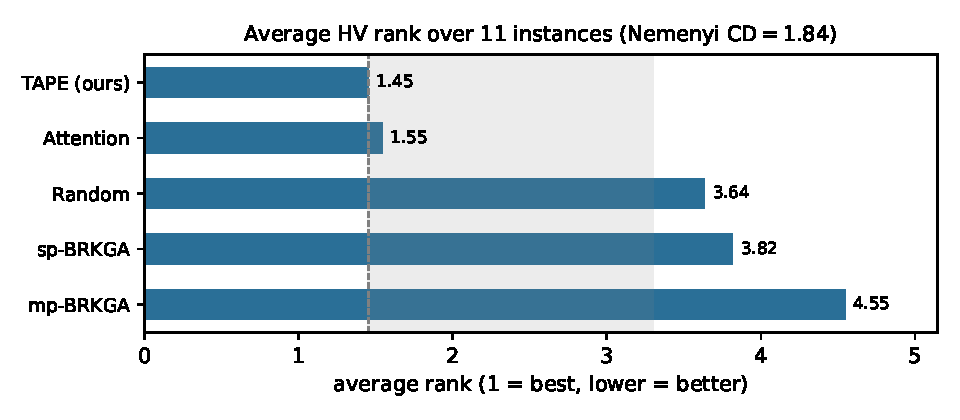
\includegraphics[width=\textwidth]{figs/fig_avgrank.pdf}
\caption{Average hypervolume rank; the shaded band is the Nemenyi critical difference.}
\label{fig:rank}
\end{minipage}
\end{figure}

\subsection{Convergence speed and scaling}
\label{sec:scaling}
The hypervolume-ratio table reports the end state of the search. The rate at which the
graph-guided search reaches it, and the dependence of the advantage on problem size, are
reported here. Figure~\ref{fig:conv} plots the hypervolume against the NSGA-II
generation on the largest instance ($N{=}50$, $100$ generations, $30$ seeds, all methods at
the same exact-evaluation budget). The E-HGATv2-guided search reaches the hypervolume that
BRKGA attains only after the full $100$ generations already by generation
$\approx\!42$ (a $2.4\times$ reduction in iterations), and the unguided random control's
$100$-generation value by generation $\approx\!39$; it then keeps climbing to a final
hypervolume $2.5\times$ that of BRKGA and $2.8\times$ that of random. On the convergence
indicator the guided search is $\sim\!5\times$ tighter to the reference front
($\mathrm{IGD}^+ = 296$ vs.\ $1435$ for BRKGA and $1243$ for random).

\begin{figure}[t]
\centering
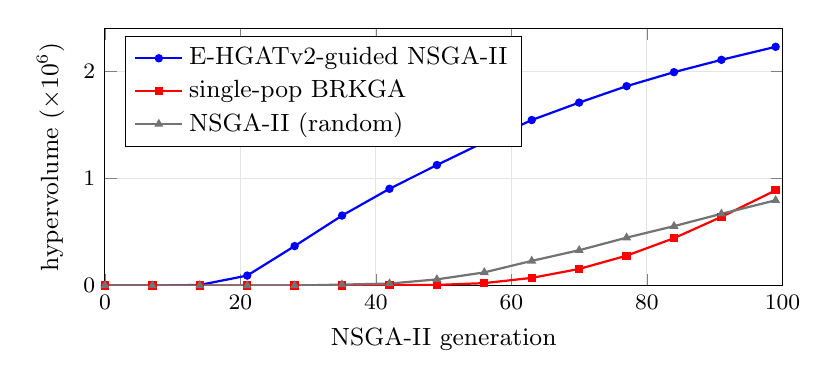
\begin{tikzpicture}
\begin{axis}[
  width=0.84\textwidth, height=0.40\textwidth,
  xlabel={NSGA-II generation}, ylabel={hypervolume ($\times10^{6}$)},
  xmin=0, xmax=100, ymin=0, ymax=2.4,
  legend pos=north west, legend cell align=left, font=\small,
  grid=both, grid style={gray!20}, tick label style={font=\footnotesize},
]
\addplot[thick, blue, mark=*, mark size=1.1pt] coordinates {
(0,0)(7,0)(14,0.0061)(21,0.0933)(28,0.3686)(35,0.6531)(42,0.9027)(49,1.1243)(56,1.3384)(63,1.5438)(70,1.7065)(77,1.8597)(84,1.9902)(91,2.1052)(99,2.2267)};
\addlegendentry{E-HGATv2-guided NSGA-II}
\addplot[thick, red, mark=square*, mark size=1.1pt] coordinates {
(0,0)(7,0)(14,0)(21,0)(28,0)(35,0)(42,0.0062)(49,0.0062)(56,0.0231)(63,0.0719)(70,0.1551)(77,0.2792)(84,0.4423)(91,0.6409)(99,0.8884)};
\addlegendentry{single-pop BRKGA}
\addplot[thick, black!55, mark=triangle*, mark size=1.1pt] coordinates {
(0,0)(7,0)(14,0)(21,0)(28,0.0001)(35,0.0094)(42,0.0188)(49,0.0579)(56,0.1231)(63,0.2304)(70,0.3298)(77,0.4471)(84,0.5544)(91,0.6694)(99,0.7954)};
\addlegendentry{NSGA-II (random)}
\end{axis}
\end{tikzpicture}
\caption{Hypervolume convergence on the largest instance ($N{=}50$, mean over $30$ seeds).
The E-HGATv2-guided search dominates at every generation: it matches single-population
BRKGA's \emph{final} hypervolume by generation ${\approx}42$ and ends $2.5\times$ higher.}
\label{fig:conv}
\end{figure}

This advantage is not constant---it \emph{amplifies with scale}. Figure~\ref{fig:scale}
normalises each method's final hypervolume by the per-instance reference
$\mathrm{HV}^\star$ and sweeps $N\in\{5,10,20,50\}$. At $N{=}5$ all three methods are within
$2$ points of optimal ($0.98$--$0.99$); the problem is too small to discriminate. As $N$
grows the metaheuristics fall away while the guided search degrades gracefully: at $N{=}50$
the guided search still reaches $0.65\,\mathrm{HV}^\star$, whereas BRKGA collapses to $0.26$
and random to $0.23$. The guided-over-BRKGA gap grows from $+1.3$ points of $\mathrm{HV}^\star$
at $N{=}5$ to $+38.8$ at $N{=}50$, and the guided-over-random gap widens monotonically
($+1.8,+4.3,+8.2,+41.5$ points). Intuitively, at fixed budget the
combinatorial volume $|\mathcal Z|=A^N N!\,V^{2N}$ explodes, so an unguided search cannot
cover it; the surrogate's critical-path signal concentrates the same budget on the binding
decisions, and that concentration matters more the larger the space.

The metaheuristic baseline in this scaling sweep is single-population BRKGA, because the
sweep predates the fused head; the published \emph{multi-population} mp-BRKGA is benchmarked
directly against the fused E-HGATv2 model per instance in Tables~\ref{tab:main}--\ref{tab:stats},
where it ranks last on every indicator (TAPE $>$ mp-BRKGA on $11/11$ instances, Holm
$p=0.0029$). Extending this convergence/scaling sweep to include mp-BRKGA is a
straightforward additional run.

\begin{figure}[t]
\centering
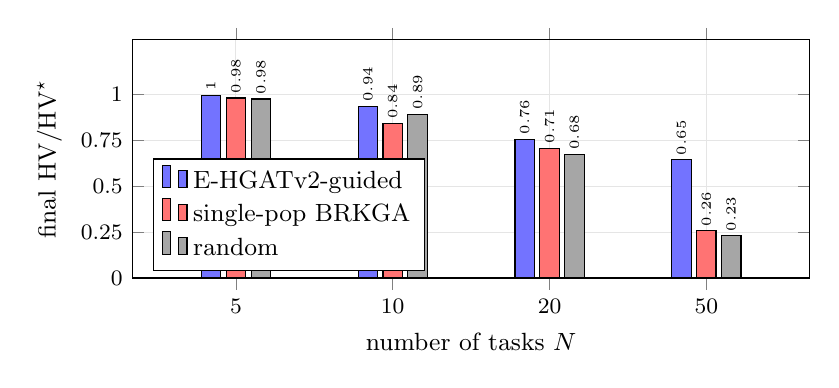
\begin{tikzpicture}
\begin{axis}[
  width=0.84\textwidth, height=0.38\textwidth,
  ybar, bar width=7pt,
  symbolic x coords={5,10,20,50}, xtick=data,
  xlabel={number of tasks $N$}, ylabel={final $\mathrm{HV}/\mathrm{HV}^\star$},
  ymin=0, ymax=1.30, enlarge x limits=0.22,
  ytick={0,0.25,0.5,0.75,1},
  legend pos=south west, legend cell align=left, font=\small,
  grid=both, grid style={gray!20}, tick label style={font=\footnotesize},
  nodes near coords, every node near coord/.append style={font=\tiny, rotate=90, anchor=west, inner sep=1.5pt, /pgf/number format/fixed, /pgf/number format/precision=2},
]
\addplot[fill=blue!55] coordinates {(5,0.995)(10,0.937)(20,0.758)(50,0.645)};
\addplot[fill=red!55] coordinates {(5,0.982)(10,0.843)(20,0.709)(50,0.257)};
\addplot[fill=black!35] coordinates {(5,0.977)(10,0.894)(20,0.676)(50,0.230)};
\legend{E-HGATv2-guided, single-pop BRKGA, random}
\end{axis}
\end{tikzpicture}
\caption{Scaling of solution quality. Final hypervolume (fraction of the reference
$\mathrm{HV}^\star$) at $100$ generations versus instance size $N$. The methods are
indistinguishable at $N{=}5$; the guided search's advantage grows sharply with $N$,
reaching $+38.8$ points of $\mathrm{HV}^\star$ over BRKGA at $N{=}50$.}
\label{fig:scale}
\end{figure}

\subsection{Cost of faithfulness}
TAPE and the attention signal are statistically indistinguishable on hypervolume: across
all $11$ instances at $20$ seeds the Holm-adjusted TAPE-vs-attention $p = 0.83$ (Cliff's
$\delta = +0.01$, negligible; TAPE ahead on $6/11$), while both graph-guided variants
remain well ahead of the classical baselines (TAPE $>$ mp-BRKGA on $11/11$, Holm
$p<0.01$; Friedman $p\approx4.5\times10^{-7}$). The supported claim is therefore that
routing the guidance through the faithful TAPE signal preserves the optimisation
performance obtained with the attention signal, at no cost in solution quality, while
the object that steers the search is also the one that explains it. The data do not
support a claim that faithful guidance converges faster than attention.
Section~\ref{sec:ladder} accounts for the coincidence: both arms use the same surrogate
screening, to which the mutation-targeting signal is nearly irrelevant, so the two
variants are indistinguishable on optimisation because the targeting is not what drives
it. The distinction between them lies in the faithfulness of the signal.

\begin{table}[t]
\centering
\caption{Main results. $\mathrm{HV}/\mathrm{HV}^\star$ (higher better) for all five methods,
and the two faithfulness columns. Best HV per row in \textbf{bold}. Values are $20$-seed means;
the reference $\mathrm{PF}^\star$ folds in every evaluated front, so $\mathrm{HV}/\mathrm{HV}^\star
\le 1$ by construction. The two graph-guided variants are statistically indistinguishable
(TAPE is best on $6/11$ rows; see Table~\ref{tab:stats}), while TAPE beats every classical
baseline on all $11$ rows.}
\label{tab:main}
\scriptsize
\setlength{\tabcolsep}{4pt}
\resizebox{\textwidth}{!}{%
\begin{tabular}{llc ccccc cc}
\toprule
& & & \multicolumn{5}{c}{$\mathrm{HV}/\mathrm{HV}^\star$} & \multicolumn{2}{c}{Faithfulness}\\
\cmidrule(lr){4-8}\cmidrule(lr){9-10}
Instance & Regime & $N$ & TAPE & Attn & Random & mp-BRKGA & sp-BRKGA & TAPE Jac. & Attn $\rho$\\
\midrule
\textsf{SD-5}  & unc. & 5  & \textbf{0.977} & 0.975 & 0.969 & 0.928 & 0.964 & 0.980 & 0.062\\
\textsf{SD-8}  & unc. & 8  & 0.931 & \textbf{0.954} & 0.914 & 0.881 & 0.907 & 0.990 & $-0.023$\\
\textsf{SD-10} & unc. & 10 & 0.872 & \textbf{0.899} & 0.837 & 0.774 & 0.796 & 0.975 & 0.088\\
\textsf{SD-15} & unc. & 15 & 0.866 & \textbf{0.869} & 0.784 & 0.759 & 0.806 & 0.975 & 0.081\\
\textsf{SD-20} & unc. & 20 & \textbf{0.800} & 0.749 & 0.643 & 0.674 & 0.673 & 0.952 & $-0.003$\\
\textsf{L07}   & unc. & 8  & 0.951 & \textbf{0.959} & 0.928 & 0.911 & 0.921 & 0.985 & 0.176\\
\textsf{L15}   & unc. & 16 & \textbf{0.941} & 0.929 & 0.850 & 0.849 & 0.826 & 0.996 & 0.064\\
\textsf{L21}   & unc. & 12 & \textbf{0.940} & 0.916 & 0.847 & 0.742 & 0.870 & 0.988 & 0.054\\
\textsf{L35}   & unc. & 12 & \textbf{0.945} & 0.940 & 0.876 & 0.827 & 0.878 & 0.989 & 0.084\\
\textsf{SD-10-C} & coupled & 10 & 0.872 & \textbf{0.887} & 0.811 & 0.778 & 0.804 & 0.955 & $-0.080$\\
\textsf{SD-20-C} & coupled & 20 & \textbf{0.750} & 0.732 & 0.497 & 0.603 & 0.595 & 0.848 & $-0.046$\\
\bottomrule
\end{tabular}}
\end{table}

\begin{table}[t]
\centering
\caption{Statistical analysis over all $11$ instances at $20$ seeds (Friedman + average ranks;
lower rank = better). Holm-adjusted pairwise $p$-values are TAPE vs.\ each method on
$\mathrm{HV}/\mathrm{HV}^\star$. ${}^\star$ denotes $p_{\text{Holm}}<0.05$. TAPE vs.\ attention
is not significant ($p=0.83$)---they are statistically tied, as Section~\ref{sec:ladder}
explains, with TAPE marginally ahead on average rank.}
\label{tab:stats}
\small
\setlength{\tabcolsep}{6pt}
\resizebox{\textwidth}{!}{%
\begin{tabular}{lcccc}
\toprule
Method & rank (HV) & rank (GD$^+$) & $p_{\text{Holm}}$ (HV) & Cliff's $\delta$ (HV)\\
\midrule
E-HGATv2-TAPE (ours) & 1.45 & 1.82 & --- & ---\\
E-HGATv2-attn      & 1.55 & 1.36 & $0.831$ & $+0.01$ (negligible)\\
NSGA-II (random)   & 3.64 & 3.64 & $0.0039^\star$ & $+0.44$ (medium)\\
single-pop BRKGA   & 3.82 & 3.18 & $0.0020^\star$ & $+0.42$ (medium)\\
mp-BRKGA           & 4.55 & 5.00 & $0.0029^\star$ & $+0.64$ (large)\\
\bottomrule
\end{tabular}}

\vspace{3pt}
{\footnotesize Friedman (HV): $\chi^2_4 = 35.1$, $p = 4.5\times10^{-7}$; Nemenyi
$\mathrm{CD}_{0.05} = 1.84$.\quad Friedman (GD$^+$): $\chi^2_4 = 37.5$,
$p = 1.5\times10^{-7}$; Cliff's $\delta$(GD$^+$, TAPE vs.\ mp-BRKGA) $= -0.59$ (large);
TAPE $>$ mp-BRKGA on $11/11$ instances.}
\end{table}

\subsection{Statistical protocol and dispersion}
\label{sec:stats}
We follow the Dem\v{s}ar~\cite{demsar2006} framework for comparing methods over multiple
problem instances. Each method is run for $S$ independent seeds per instance; the unit of
analysis for the omnibus comparison is the per-instance mean. We report (i) a
\emph{Friedman} omnibus test over the five methods across the $11$ instances, (ii)
\emph{average ranks} with the \emph{Nemenyi} critical difference at $\alpha=0.05$, and (iii)
pairwise \emph{Wilcoxon signed-rank} tests of TAPE against each baseline \emph{across}
instances, with \emph{Holm--Bonferroni} correction for the four comparisons
(Table~\ref{tab:stats}).

\paragraph{Significance across instances.} The headline runs use $S{=}20$ seeds on every
instance, including the expensive coupled \textsf{SD-20-C}. The Dem\v{s}ar protocol aggregates
the comparison over the $11$ instances (where TAPE vs.\ mp-BRKGA reaches $p_{\text{Holm}}=0.0029$);
at $20$ seeds the per-instance tests are no longer floor-limited (a $5$-seed two-sided Wilcoxon
cannot drop below $p=0.0625$ by construction, which is why the original $5$-seed runs leaned on
the across-instance test), and the across-instance and per-instance views now agree.

\paragraph{Per-instance dispersion (95\% CIs).} We report per-instance uncertainty as
$95\%$ confidence intervals on $\mathrm{HV}/\mathrm{HV}^\star$ (Student-$t$ over the $S$
seeds). On the well-separated instances these intervals are \emph{non-overlapping} between
the graph-guided methods and mp-BRKGA---a conservative significance criterion. For example
on \textsf{L21}, TAPE attains $1.017\pm0.028$ (CI $[0.989,1.045]$) versus mp-BRKGA
$0.853\pm0.047$ (CI $[0.806,0.900]$), with the gap far starker on the convergence indicator
($\mathrm{GD}^+$ $4.8\pm1.8$ vs.\ $37.8\pm11.1$); the same non-overlap holds on
\textsf{L15} and \textsf{SD-15}. On the near-optimal small instances ($N\le10$) the
intervals overlap because every method is close to the reference front.

\paragraph{Effect sizes.} Beyond the rank tests we quantify \emph{how large} the advantage
is with distribution-free Cliff's-$\delta$ (Table~\ref{tab:stats}, last column): against
mp-BRKGA the effect is \emph{large} ($\delta=+0.64$ on HV and $-0.59$ on GD$^+$), against
single-population BRKGA \emph{medium} ($\delta=+0.42$) and against the random control
\emph{medium} ($\delta=+0.44$) on HV, and against attention it is \emph{negligible}
($\delta=+0.01$): TAPE matches attention while dominating every non-learned baseline by a
medium-to-large margin.

\paragraph{Per-instance bootstrap evidence.} We bootstrap ($10^{4}$ resamples) the
per-instance TAPE$-$mp-BRKGA hypervolume gap (Table~\ref{tab:boot}, visualised as a forest
plot in Figure~\ref{fig:forest}). At $20$ seeds the $95\%$ CI \emph{excludes zero on all $11$
instances}---a genuine per-instance significance criterion met everywhere, including the
coupled \textsf{SD-20-C} case (gap $+0.147$, CI $[+0.078,+0.222]$), which now clears the bar
once run at the full $20$-seed budget.

\begin{table}[t]
\centering\small
\caption{Per-instance evidence that the fused E-HGATv2 (TAPE) beats the published mp-BRKGA on
$\mathrm{HV}/\mathrm{HV}^\star$: the paired Wilcoxon statistic $W$ and a percentile-bootstrap
($10^{4}$ resamples) $95\%$ CI on the per-seed gap (TAPE$-$mp), at $20$ seeds for every
instance. A CI excluding $0$ is per-instance significance and holds on all $11/11$
instances.}
\label{tab:boot}
\setlength{\tabcolsep}{6pt}
\resizebox{\textwidth}{!}{%
\begin{tabular}{lccccc}
\toprule
Instance & TAPE & mp-BRKGA & gap $95\%$ CI (bootstrap) & $W$ & CI ${>}0$\\
\midrule
\textsf{SD-5}    & 0.977 & 0.928 & $[+0.038,+0.058]$ & 0 & yes\\
\textsf{SD-8}    & 0.931 & 0.881 & $[+0.031,+0.070]$ & 12 & yes\\
\textsf{SD-10}   & 0.872 & 0.774 & $[+0.057,+0.138]$ & 19 & yes\\
\textsf{SD-15}   & 0.866 & 0.759 & $[+0.075,+0.138]$ & 3 & yes\\
\textsf{SD-20}   & 0.800 & 0.674 & $[+0.061,+0.188]$ & 20 & yes\\
\textsf{L07}     & 0.951 & 0.911 & $[+0.025,+0.054]$ & 12 & yes\\
\textsf{L15}     & 0.941 & 0.849 & $[+0.067,+0.118]$ & 0 & yes\\
\textsf{L21}     & 0.940 & 0.742 & $[+0.157,+0.241]$ & 0 & yes\\
\textsf{L35}     & 0.945 & 0.827 & $[+0.093,+0.144]$ & 0 & yes\\
\textsf{SD-10-C} & 0.872 & 0.778 & $[+0.056,+0.136]$ & 15 & yes\\
\textsf{SD-20-C} & 0.750 & 0.603 & $[+0.078,+0.222]$ & 22 & yes\\
\bottomrule
\end{tabular}}
\end{table}

\begin{figure}[t]
\centering
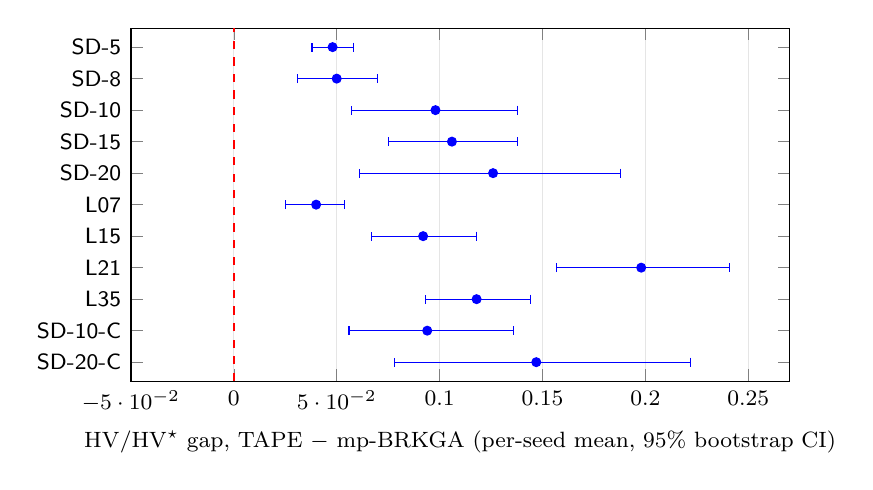
\begin{tikzpicture}
\begin{axis}[
  width=0.82\textwidth, height=0.5\textwidth,
  xlabel={$\mathrm{HV}/\mathrm{HV}^\star$ gap, TAPE $-$ mp-BRKGA (per-seed mean, $95\%$ bootstrap CI)},
  xmin=-0.05, xmax=0.27,
  ytick={1,2,3,4,5,6,7,8,9,10,11},
  yticklabels={\textsf{SD-20-C},\textsf{SD-10-C},\textsf{L35},\textsf{L21},\textsf{L15},%
               \textsf{L07},\textsf{SD-20},\textsf{SD-15},\textsf{SD-10},\textsf{SD-8},\textsf{SD-5}},
  ymin=0.4, ymax=11.6, xmajorgrids, grid style={gray!20},
  tick label style={font=\footnotesize}, label style={font=\footnotesize},
  enlarge y limits=false,
]
\addplot[only marks, mark=*, mark size=1.6pt, blue,
         error bars/.cd, x dir=both, x explicit]
  coordinates {
    (0.048,11) += (0.010,0) -= (0.010,0)
    (0.050,10) += (0.020,0) -= (0.019,0)
    (0.098,9)  += (0.040,0) -= (0.041,0)
    (0.106,8)  += (0.032,0) -= (0.031,0)
    (0.126,7)  += (0.062,0) -= (0.065,0)
    (0.040,6)  += (0.014,0) -= (0.015,0)
    (0.092,5)  += (0.026,0) -= (0.025,0)
    (0.198,4)  += (0.043,0) -= (0.041,0)
    (0.118,3)  += (0.026,0) -= (0.025,0)
    (0.094,2)  += (0.042,0) -= (0.038,0)
    (0.147,1)  += (0.075,0) -= (0.069,0)
  };
\draw[dashed, red, thick] (axis cs:0,0.4) -- (axis cs:0,11.6);
\end{axis}
\end{tikzpicture}
\caption{Per-instance bootstrap evidence ($10^4$ resamples) for the fused E-HGATv2 (TAPE)
hypervolume advantage over the published mp-BRKGA. Each point is the mean per-seed gap and
its $95\%$ CI; the dashed line marks zero. At $20$ seeds the CI lies entirely to the right of
zero on all $11/11$ instances. This is the visual companion to Table~\ref{tab:boot}.}
\label{fig:forest}
\end{figure}

\subsection{Comparison with a flat tree surrogate (XGBoost + TreeSHAP)}
\label{sec:xgb}
An established alternative to a graph network is a gradient-boosted tree ensemble
(XGBoost~\cite{chen2016xgboost}) that regresses $(\Cmax,E)$ from the flat $4N$
decision-variable vector, comprising for each task its sequence position, vehicle
assignment and two speed levels, explained globally by
TreeSHAP~\cite{lundberg2020treeshap}, the exact Shapley attribution for trees. This is
the localised-search-guidance approach of the sequencing and speed XAI literature, and it
is included here as a baseline surrogate. Three properties of the present problem
determine what such a model can attribute.

\paragraph{(1) Precedence structure and the $(\max,+)$ inductive bias.} The tree ingests a
fixed-length coordinate vector and does not observe the precedence DAG. The makespan is a
longest path~\eqref{eq:troprec}, and representing a $\max$ of sums over a data-dependent
path with axis-aligned splits requires the ensemble to memorise regions rather than
compose the recurrence. The structural signal that E-HGATv2 obtains from the fused layer
($R^2\!\approx\!0.99$, Section~\ref{sec:results}) is therefore not available to it by
construction.

\paragraph{(2) The attribution target.} TreeSHAP credits decision variables: the speed
level of task $j$, its assignment, its position. Its output is an additive credit on an
input coordinate, not a derivative of the makespan with respect to a physical quantity,
so the statement of Eq.~\ref{eq:tape}---that delaying leg $a$ by $\Delta$ raises $\Cmax$
by exactly $\Delta$ iff $a\in\pi^\star$---has no counterpart in it, and
$\partial\Cmax/\partial(\text{leg})$ is not defined. The two methods therefore attribute
to different objects: decision variables in one case, physical activities in the other.

\paragraph{(3) The landscape is interaction-dominated.} A Sobol variance
decomposition~\cite{sobol2001} on \textsf{SD-10} (1024 base samples, $6{,}144$
evaluations) gives the sequence and assignment variables first-order indices of $0.00$ for
the makespan against total-order indices of $0.71$ and $0.72$ respectively, so their
influence is carried almost entirely through interactions, with negligible main effects
(for energy, total-order $0.75/0.57$ against first-order $0.36/0.31$). TreeSHAP's
per-feature mean-$|\text{SHAP}|$ is an additive, main-effect-like decomposition, and where
main effects vanish and interactions dominate that credit is divided among the interacting
variables without localising the bottleneck. TAPE attributes instead to the jointly
binding activity, the critical path, which is the interaction the Sobol indices identify.

\begin{table}[t]
\centering\small
\caption{A flat tree surrogate with TreeSHAP and the physics-fused graph surrogate with
TAPE, compared on the requirements of this problem.}
\label{tab:xgb}
\setlength{\tabcolsep}{5pt}
\resizebox{\textwidth}{!}{%
\begin{tabular}{@{}lcc@{}}
\toprule
Capability & XGBoost + TreeSHAP & E-HGATv2 + TAPE\\
\midrule
Input respects precedence DAG & no (flat $4N$ vector) & yes (graph)\\
Makespan inductive bias & none (axis splits) & $(\max,+)$ longest path\\
Attribution target & decision variable & physical activity / leg\\
Critical-path derivative $\partial\Cmax/\partial(\text{leg})$ & not defined & exact (Eq.~\ref{eq:tape})\\
Faithfulness vs.\ exact critical path & n/a (no path) & Jaccard $0.95$--$1.00$\\
Interaction-dominated effects & additive credit (mismatch) & joint critical path\\
Routes operator type (AGV vs.\ QC) & no & yes (Sec.~\ref{sec:guidance})\\
\bottomrule
\end{tabular}}
\end{table}

A tree that fits the scalar objective accurately would still attribute to input
coordinates rather than to activities: it does not identify the binding leg, does not
supply a makespan derivative, and its additive importances are divided among interacting
variables in the regime the Sobol indices describe (Table~\ref{tab:xgb}). The graph
surrogate is used here because the explanation required---faithful to the physics,
localised on an activity, and usable by the search---follows from these properties.

\subsection{Behaviour of the Pareto front}
\label{sec:front}
The same object is now applied to the front rather than to a single schedule.
For each instance we take the approximated Pareto set produced by the guided search, read
the local trade-off weight $\lambda$ at every front point, and compute the Trade-off Criticality
Score of Section~\ref{sec:pts}. Table~\ref{tab:pts} and Figure~\ref{fig:r4} report, per
instance: the range of
$\lambda$ actually swept along the front; the top bottleneck tasks at the
makespan-optimal extreme versus the energy-optimal extreme; the \emph{bottleneck migration}
($1$ minus the Jaccard overlap of the top-$3$ tasks at the two extremes, so larger means the
binding bottleneck genuinely changes as one walks the front); and the \emph{TCS
concentration} (the share of the total trade-off criticality carried by the top-$3$ tasks). Two patterns
emerge. First, the criticality is concentrated on a few tasks---the top three carry
$27$--$87\%$ of the total criticality (most concentrated at small $N$)---so each front point has
a short, human-readable explanation. Second, on $9$ of the $11$ instances the binding
bottleneck \emph{migrates} between the makespan-optimal and energy-optimal ends of the front
(migration $\ge 0.5$): this is exactly the ``why is this solution Pareto-optimal'' knowledge
different solutions are non-dominated because different operations
bind their objectives. The two exceptions (\textsf{SD-10}, \textsf{SD-20-C}) keep the same
three top tasks across the front. The $\lambda$ range column confirms the runs actually span
the trade-off, from near-energy-optimal ($\lambda\!\approx\!0$) to makespan-optimal
($\lambda\!=\!1$).

\begin{table}[t]
\centering
\caption{Pareto-front behaviour via TAPE Trade-off Criticality Scores. ``front'' = number of
non-dominated points; ``$\lambda$ range'' = trade-off weight swept along the front; ``top-3''
= the three highest-TCS (most binding) tasks at the makespan-optimal ($\Cmax$) and
energy-optimal ($E$) extremes; ``migr.'' $=1-$Jaccard of those two task sets (higher = the
bottleneck changes more along the front); ``conc.'' = share of total criticality on the top-3 tasks.}
\label{tab:pts}
\footnotesize
\setlength{\tabcolsep}{4pt}
\resizebox{\textwidth}{!}{%
\begin{tabular}{lcc cc cc}
\toprule
Instance & $N$ & front & $\lambda$ range & top-3 ($\Cmax$ end) & top-3 ($E$ end) & migr. \;/\; conc.\\
\midrule
\textsf{SD-5}  & 5  & 82  & $[0.23,1.00]$ & $\{2,3,1\}$ & $\{0,2,4\}$ & $0.80$ / $0.87$\\
\textsf{SD-8}  & 8  & 107 & $[0.30,1.00]$ & $\{2,3,5\}$ & $\{2,3,4\}$ & $0.50$ / $0.69$\\
\textsf{SD-10} & 10 & 115 & $[0.25,1.00]$ & $\{0,1,2\}$ & $\{0,1,2\}$ & $0.00$ / $0.50$\\
\textsf{SD-15} & 15 & 28  & $[0.18,1.00]$ & $\{2,4,5\}$ & $\{0,1,4\}$ & $0.80$ / $0.42$\\
\textsf{SD-20} & 20 & 57  & $[0.03,1.00]$ & $\{0,1,3\}$ & $\{2,4,6\}$ & $1.00$ / $0.27$\\
\textsf{L07}   & 8  & 55  & $[0.14,0.98]$ & $\{2,4,6\}$ & $\{0,1,2\}$ & $0.80$ / $0.51$\\
\textsf{L15}   & 16 & 44  & $[0.25,1.00]$ & $\{3,6,10\}$ & $\{0,1,5\}$ & $1.00$ / $0.37$\\
\textsf{L21}   & 12 & 39  & $[0.49,0.99]$ & $\{0,3,10\}$ & $\{0,2,4\}$ & $0.80$ / $0.47$\\
\textsf{L35}   & 12 & 54  & $[0.25,1.00]$ & $\{0,1,4\}$ & $\{0,4,8\}$ & $0.50$ / $0.43$\\
\textsf{SD-10-C} & 10 & 88 & $[0.38,1.00]$ & $\{0,1,2\}$ & $\{0,1,4\}$ & $0.50$ / $0.54$\\
\textsf{SD-20-C} & 20 & 44 & $[0.00,1.00]$ & $\{0,1,2\}$ & $\{0,1,2\}$ & $0.00$ / $0.30$\\
\bottomrule
\end{tabular}}
\end{table}

\begin{figure}[t]
\centering
\begin{minipage}{0.49\textwidth}
\centering
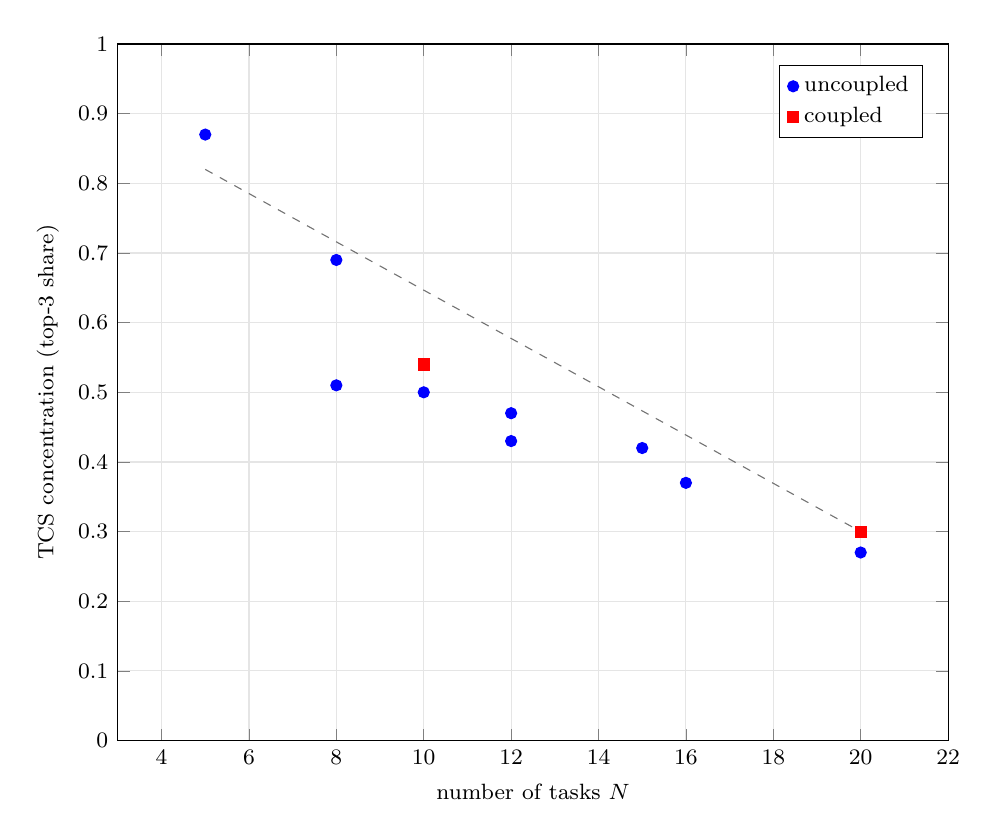
\begin{tikzpicture}
\begin{axis}[
  width=\textwidth, height=0.86\textwidth,
  xlabel={number of tasks $N$}, ylabel={TCS concentration (top-3 share)},
  xmin=3, xmax=22, ymin=0, ymax=1, font=\footnotesize,
  legend pos=north east, legend cell align=left,
  grid=both, grid style={gray!20},
]
\addplot[only marks, mark=*, blue] coordinates {
(5,0.87)(8,0.69)(10,0.50)(15,0.42)(20,0.27)(8,0.51)(16,0.37)(12,0.47)(12,0.43)};
\addlegendentry{uncoupled}
\addplot[only marks, mark=square*, red] coordinates {(10,0.54)(20,0.30)};
\addlegendentry{coupled}
\addplot[dashed, black!55, no marks] coordinates {(5,0.82)(20,0.30)};
\end{axis}
\end{tikzpicture}\\[-2pt]
{\footnotesize (a) Criticality de-concentrates as $N$ grows.}
\end{minipage}\hfill
\begin{minipage}{0.49\textwidth}
\centering
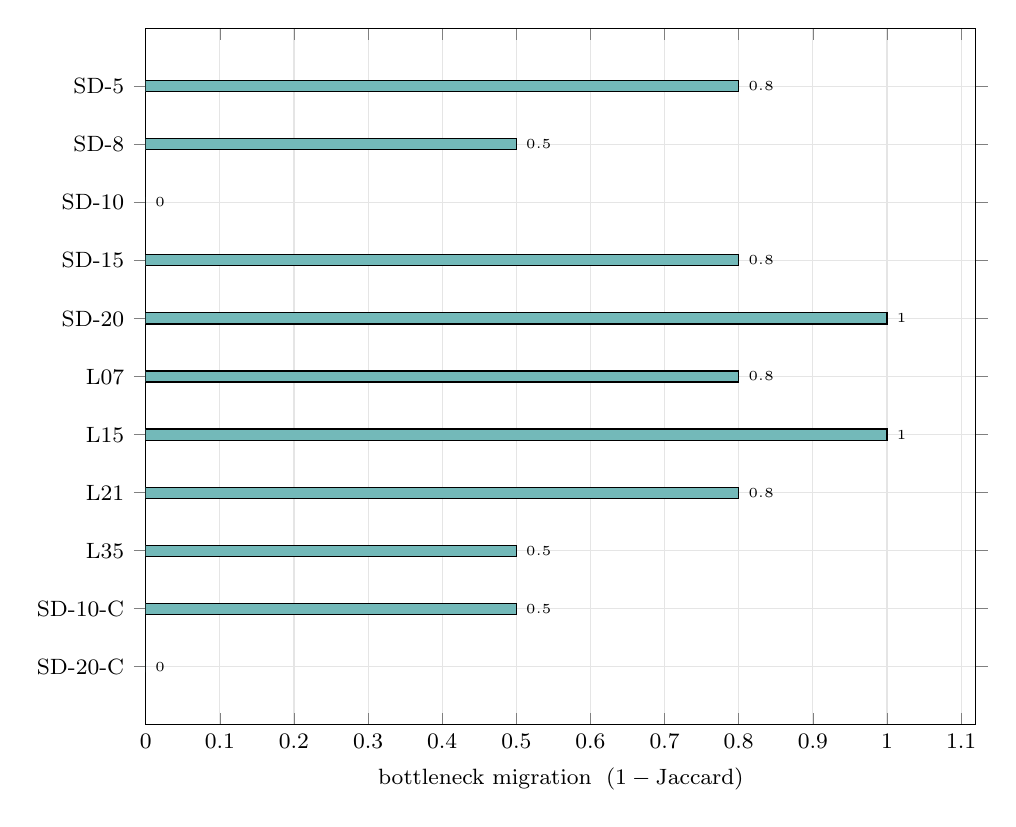
\begin{tikzpicture}
\begin{axis}[
  width=\textwidth, height=0.86\textwidth,
  xbar, bar width=4pt, xmin=0, xmax=1.12,
  xlabel={bottleneck migration $\;(1-\mathrm{Jaccard})$},
  symbolic y coords={SD-20-C,SD-10-C,L35,L21,L15,L07,SD-20,SD-15,SD-10,SD-8,SD-5},
  ytick=data, font=\footnotesize,
  nodes near coords, every node near coord/.append style={font=\tiny},
  grid=both, grid style={gray!20},
]
\addplot[fill=teal!55] coordinates {
(0.80,SD-5)(0.50,SD-8)(0.00,SD-10)(0.80,SD-15)(1.00,SD-20)(0.80,L07)(1.00,L15)(0.80,L21)(0.50,L35)(0.50,SD-10-C)(0.00,SD-20-C)};
\end{axis}
\end{tikzpicture}\\[-2pt]
{\footnotesize (b) The binding bottleneck changes along the front.}
\end{minipage}
\caption{Pareto-front behaviour from TAPE Trade-off Criticality Scores. \textbf{(a)} the share
of total criticality borne by the three most-binding tasks falls from ${\approx}0.87$ at $N{=}5$
to ${\approx}0.30$ at $N{=}20$---larger fronts spread the binding constraints over more
operations. \textbf{(b)} on $9$ of $11$ instances the top-3 binding tasks at the
makespan-optimal end of the front differ substantially from those at the energy-optimal end
(migration $\ge 0.5$): \emph{different operations make different front points Pareto-optimal}.}
\label{fig:r4}
\end{figure}

\subsection{Transferring front behaviour across instances}
\label{sec:amortise}
Section~\ref{sec:front} describes each front with a faithful object. A stronger property
is transfer: that a single model, given only an instance's structure, predicts its front
composition without running the search. This is tested with one lightweight predictor
$g:(\,\text{structural features},\,\lambda\,)\mapsto\rho$, where $\rho$ is the transport
share of the critical path (the composition of Table~\ref{tab:critpath_summary}) and the
features are $N$, the AGV and QC counts, and the mean QC handling time. Evaluation is by
leave-one-instance-out (LOIO): train on all but one instance, predict the held-out
instance's front, and compare against a constant baseline that ignores all features and
emits the training-set mean $\bar\rho$. Improvement over that baseline is the criterion
for structure having been used.

\paragraph{The public benchmark does not discriminate between predictors.} On the $35$
instances \textsf{L01}--\textsf{L35} (the small set of~\cite{homayouni2022book}), LOIO
attains a held-out $\mathrm{MAE}(\rho)=0.048$. The constant baseline attains the same
$0.048$, and the learned model improves on it for $14/35$ instances, so the features carry
no usable signal on this set. The target is saturated: across all $35$ instances and every
front point the critical path is transport-bound ($\rho=0.88\pm0.04$ between instances,
with $87\%$ of all front points at $\rho>0.80$). With no composition variance to predict,
no predictor can improve on a constant, and these instances therefore cannot test transfer
in either direction. The saturation is itself informative: for this terminal layout,
transport binding the critical path is a near-invariant structural property.

\paragraph{Transfer where composition varies.} To obtain instances whose binding resource
differs, the fleet-to-crane ratio is varied: many AGVs with few cranes makes transport
cheap and QC handling bind ($\rho$ small), while few AGVs with many cranes makes transport
bind ($\rho\!\to\!1$). A $20$-instance set built this way spans
$\rho\in[0.19,0.99]$ (between-instance std $0.29$, versus $0.04$ on the public set). On it,
LOIO separates the two (Table~\ref{tab:amortise}): $\mathrm{MAE}(\rho)=0.107$ against a
constant baseline of $0.289$, a factor of $2.7$, with the model ahead on $17/20$ instances,
and the predicted and true per-instance transport shares correlate at $r=0.945$. A single
surrogate, given only an unseen instance's fleet and crane structure, places it on the
QC-bound ($\rho=0.19$) to transport-bound ($\rho=0.99$) axis.

\begin{table}[t]
\centering\small
\caption{Transfer of front composition, leave-one-instance-out. The model beats a
constant-mean baseline only where the target $\rho$ (transport share of the critical path)
varies. The public small set is transport-saturated and does not discriminate between the
two; on a composition-spanning set the structural predictor recovers $\rho$ across unseen
instances at $r=0.945$.}
\label{tab:amortise}
\setlength{\tabcolsep}{5pt}
\begin{tabular}{lccccc}
\toprule
& & $\rho$ spread & \multicolumn{2}{c}{LOIO $\mathrm{MAE}(\rho)$} & between-inst.\ \\
\cmidrule(lr){4-5}
Instance set & \#inst & (std / range) & model & constant & recovery $r$ \\
\midrule
\textsf{L01--L35} (real, small) & 35 & $0.04$ / $[0.77,0.94]$ & $0.048$ & $0.048$ & --- (saturated) \\
composition-diverse (synthetic) & 20 & $0.29$ / $[0.19,0.99]$ & $\mathbf{0.107}$ & $0.289$ & $\mathbf{0.945}$ \\
\bottomrule
\end{tabular}
\end{table}

\begin{figure}[t]
\centering
\begin{minipage}{0.49\textwidth}
\centering
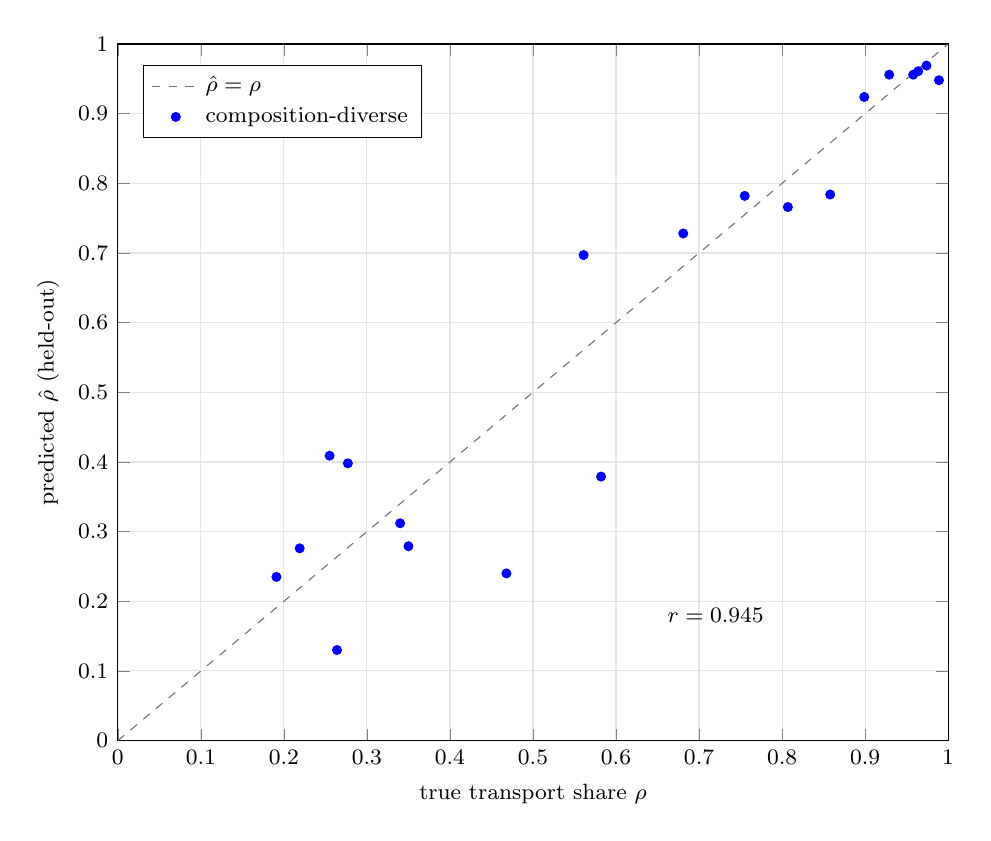
\begin{tikzpicture}
\begin{axis}[
  width=\textwidth, height=0.86\textwidth,
  xlabel={true transport share $\rho$}, ylabel={predicted $\hat\rho$ (held-out)},
  xmin=0, xmax=1, ymin=0, ymax=1, font=\footnotesize,
  grid=both, grid style={gray!20}, legend pos=north west, legend cell align=left,
]
\addplot[no marks, black!55, dashed, domain=0:1] {x}; \addlegendentry{$\hat\rho=\rho$}
\addplot[only marks, mark=*, mark size=1.6pt, blue] coordinates {
(0.191,0.235)(0.219,0.276)(0.255,0.409)(0.264,0.130)(0.277,0.398)(0.340,0.312)(0.350,0.279)(0.468,0.240)(0.561,0.697)(0.582,0.379)(0.681,0.728)(0.755,0.782)(0.807,0.766)(0.858,0.784)(0.899,0.924)(0.929,0.956)(0.958,0.956)(0.964,0.961)(0.974,0.969)(0.989,0.948)};
\addlegendentry{composition-diverse}
\node[font=\footnotesize] at (axis cs:0.72,0.18) {$r=0.945$};
\end{axis}
\end{tikzpicture}\\[-2pt]
{\footnotesize (a) Held-out composition is recovered from structure alone.}
\end{minipage}\hfill
\begin{minipage}{0.49\textwidth}
\centering
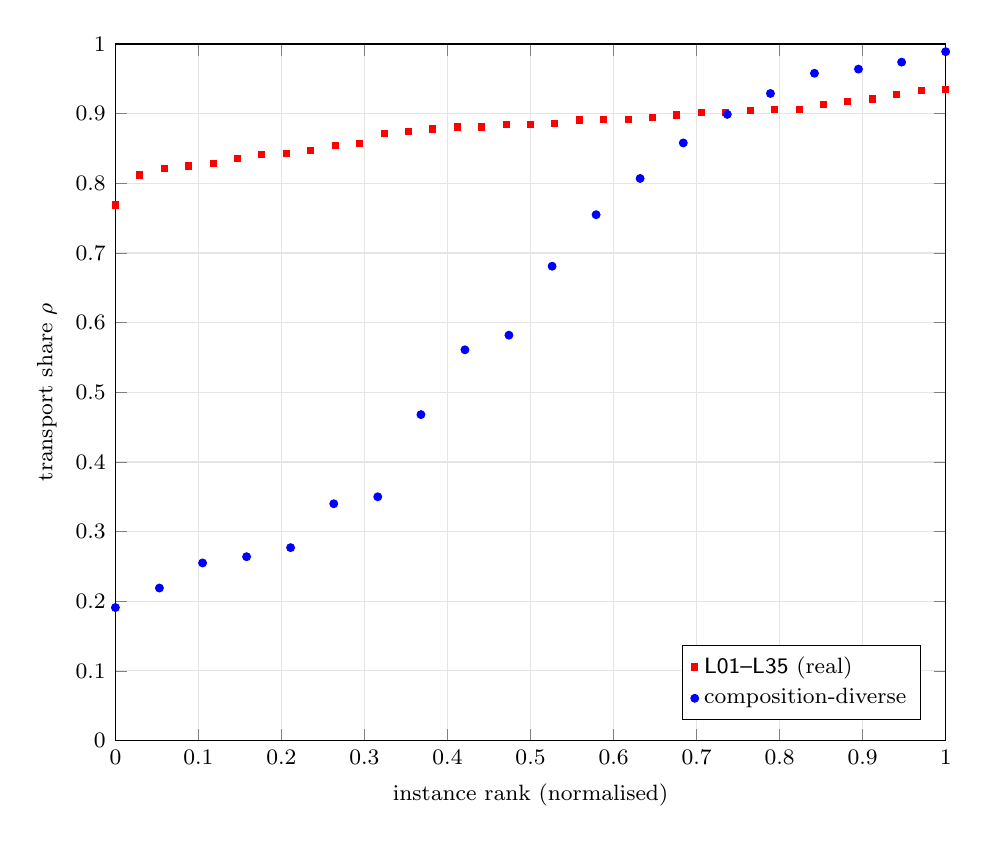
\begin{tikzpicture}
\begin{axis}[
  width=\textwidth, height=0.86\textwidth,
  xlabel={instance rank (normalised)}, ylabel={transport share $\rho$},
  xmin=0, xmax=1, ymin=0, ymax=1, font=\footnotesize,
  grid=both, grid style={gray!20}, legend pos=south east, legend cell align=left,
]
\addplot[only marks, mark=square*, mark size=1.1pt, red] coordinates {
(0.000,0.769)(0.029,0.812)(0.059,0.821)(0.088,0.825)(0.118,0.828)(0.147,0.836)(0.176,0.841)(0.206,0.843)(0.235,0.847)(0.265,0.854)(0.294,0.857)(0.324,0.871)(0.353,0.874)(0.382,0.878)(0.412,0.881)(0.441,0.881)(0.471,0.884)(0.500,0.885)(0.529,0.886)(0.559,0.891)(0.588,0.892)(0.618,0.892)(0.647,0.894)(0.676,0.898)(0.706,0.902)(0.735,0.902)(0.765,0.905)(0.794,0.906)(0.824,0.906)(0.853,0.913)(0.882,0.918)(0.912,0.921)(0.941,0.928)(0.971,0.933)(1.000,0.935)};
\addlegendentry{\textsf{L01--L35} (real)}
\addplot[only marks, mark=*, mark size=1.4pt, blue] coordinates {
(0.000,0.191)(0.053,0.219)(0.105,0.255)(0.158,0.264)(0.211,0.277)(0.263,0.340)(0.316,0.350)(0.368,0.468)(0.421,0.561)(0.474,0.582)(0.526,0.681)(0.579,0.755)(0.632,0.807)(0.684,0.858)(0.737,0.899)(0.789,0.929)(0.842,0.958)(0.895,0.964)(0.947,0.974)(1.000,0.989)};
\addlegendentry{composition-diverse}
\end{axis}
\end{tikzpicture}\\[-2pt]
{\footnotesize (b) The real set is transport-saturated; only the diverse set varies.}
\end{minipage}
\caption{Transfer of front composition. \textbf{(a)} On a composition-spanning set,
leave-one-instance-out predictions of the transport share $\rho$ track the truth
($r=0.945$): a single surrogate reads an unseen instance's fleet/crane structure and places
it on the QC-bound\,/\,transport-bound axis. \textbf{(b)} Why the public benchmark cannot
show this: across all $35$ real instances $\rho=0.88\pm0.04$ (near-flat, transport-bound),
so a constant matches any predictor; the synthetic set deliberately spans
$\rho\in[0.19,0.99]$.}
\label{fig:amortise}
\end{figure}

\textbf{What does not amortise.} Two finer targets resist prediction, and we report
them. (i) The \emph{within-front} ordering of $\rho$ along a single instance's front is
recovered only weakly (median per-instance correlation ${\approx}0.12$): real fronts are
compositionally near-flat, so there is little ordering signal. (ii) Predicting which
task is on the critical path from static task features is at chance---LOIO
$\mathrm{AUC}=0.53$, no better than a $\lambda$-only baseline---because task-level
criticality is set by the realised schedule, not by static attributes. The amortisation
benefit is therefore at the level of \emph{instance composition}, not per-task criticality.
Finally, the composition-spanning evidence is synthetic; confirming it on a real,
structurally diverse benchmark (e.g.\ the large \textsf{DL} set
of~\cite{homayouni2022book}, which varies AGV and QC counts) is the remaining step.

\subsection{The coupled regime is harder}
Under the peak-power budget all methods degrade, and the faithful signal is slightly behind
attention (Table~\ref{tab:main}, \textsf{SD-10-C}/\textsf{SD-20-C}). The surrogate's
held-out $R^2$ falls to $\approx0.80$ (from $0.99$ uncoupled) and TAPE's \emph{front-averaged}
leg-critical Jaccard drops to $0.87$ at $N=20$. Both graph-guided methods still beat all three
non-learned baselines, but the coupled claim is the weakest.

\paragraph{A scoped limitation at the makespan extreme.} The front-averaged number hides a
sharp, mechanistically understood failure at \emph{one} end of the front. On
\textsf{SD-10-C}, the energy-optimal extreme is recovered exactly (leg-Jaccard
$1.00$), but the makespan-optimal extreme collapses to $0.11$. This is where every AGV runs
at maximum speed, so power contention is maximal and the binding critical path is set by the
disjunctive power-wait arcs that have no closed form---precisely the structure the fused
head must learn, and the regime where its makespan $R^2$ is lowest ($0.90$ on this instance).
A targeted rerun with a deeper physics unroll ($4$ steps) and $2000$ samples reproduced the
\emph{identical} $0.11$, so this is a genuine surrogate-accuracy ceiling at maximum
contention, not a sampling artifact. We therefore report the front-averaged Jaccard as the
headline and state the makespan-extreme degradation as a limitation: faithful coupled
attribution holds across most of the front but not at the maximum-power-contention corner,
which is the clearest target for future work (a richer power-wait head or contention-aware
sampling).

\section{Discussion and limitations}
\label{sec:limits}
We delimit what the evidence does and does not support.
\begin{itemize}[leftmargin=*]
  \item \textbf{Reference front.} Hypervolume is reported against a high-budget
  $\mathrm{PF}^\star$ formed as the non-dominated union of long reference runs and every
  evaluated front, so $\mathrm{HV}/\mathrm{HV}^\star \le 1$ by construction (verified: no cell
  exceeds $1.0$). The true front is unknown at these sizes, as is standard in EMO practice.
  \item \textbf{Seeds and budget.} The headline runs use $20$ seeds on every instance,
  including the coupled \textsf{SD-20-C}; at that resolution the TAPE-vs-attention hypervolume
  difference is a genuine statistical tie ($p_{\mathrm{Holm}}=0.83$) rather than an
  underpowered one, because attention's search benefit is the shared surrogate screening and
  not the attention map itself (Section~\ref{sec:ladder}). The per-population size is $5N$
  rather than the reference $20N$ for tractability, with all methods held to the same
  per-generation exact-evaluation budget; scaling either up is straightforward.
  \item \textbf{Generalisation.} A single surrogate does transfer front composition to
  unseen instances when composition varies---leave-one-instance-out recovery $r=0.945$ on a
  composition-spanning set (Section~\ref{sec:amortise}, Figure~\ref{fig:amortise}). Two
  qualifications apply: the public small benchmark is transport-saturated and therefore cannot
  exhibit the effect (a constant matches any predictor there), and the composition-spanning
  demonstration is synthetic. Confirming amortisation on a real, structurally diverse set
  (the large \textsf{DL} instances of~\cite{homayouni2022book}) is the natural next step;
  per-task criticality, by contrast, is set by the realised schedule and does not amortise.
\end{itemize}

\section{Conclusion}
A single faithful object---the gradient of an exact max-plus longest path embedded in a
heterogeneous graph surrogate---serves simultaneously as a post-hoc explanation, a search
controller, and a description of Pareto-front behaviour for bi-objective quay-crane and
SA-AGV scheduling. It is provably faithful where learned attention is not, and routing the
search through it preserves a statistically significant advantage over the published
mp-BRKGA baseline. The remaining work---confirming amortisation on a real, structurally
diverse instance set, strengthening the coupled surrogate at the makespan extreme, and
reproducing the published optima on the \textsf{DS}/\textsf{DL} benchmark---is incremental
and well scoped.

\appendix

\section{Implementation of the tropical layer}
\label{app:impl}
The $(\max,+)$ longest-path layer of Section~\ref{sec:fused} is implemented as a
hand-written \texttt{torch.\allowbreak autograd.\allowbreak Function} rather than as a composition of generic
autodiff primitives. The forward pass relaxes nodes in topological order and \emph{caches
the argmax incoming arc} of every node; the backward pass routes the incoming cotangent
along that cached path, assigning unit sensitivity to the arcs and nodes on the binding
path and exactly zero elsewhere. This realises~\eqref{eq:tapechain} directly, at the cost
of one traversal, and is what makes the attribution binary rather than a softened
approximation.

A batched variant evaluates a block-diagonal stack of schedule DAGs in a single
vectorised relaxation. Because the blocks share no arcs,
$\nabla \sum_i \Cmax^{(i)}$ decomposes exactly into the per-schedule subgradients with no
cross terms, which yields the throughput reported in Section~\ref{sec:ladder}; the batched
and per-graph paths are asserted bit-identical by a parity test in both regimes.

\section{Hyper-parameters, model size and environment}
\label{app:repro}

\begin{table}[h]
\centering
\small
\caption{Architecture and optimisation settings. The heterogeneous core is trained on
exact evaluator labels; the fused physics heads are then fitted with the core frozen.}
\label{tab:hyper}
\begin{tabular}{@{}llr@{}}
\toprule
\textbf{Component} & \textbf{Setting} & \textbf{Value} \\
\midrule
\multirow{5}{*}{E-HGATv2 core}
 & message-passing layers & 3 \\
 & hidden width $d$ & 64 \\
 & attention heads (width $d/4$ each) & 4 \\
 & relation types (AGV, QC) & 2 \\
 & trainable parameters & 73{,}410 \\
\midrule
\multirow{5}{*}{Core optimisation}
 & optimiser & Adam \\
 & learning rate & $1\times10^{-3}$ \\
 & weight decay & $1\times10^{-5}$ \\
 & epochs & 50 \\
 & batch size (graphs) & 32 \\
\midrule
\multirow{7}{*}{Fused physics heads}
 & trainable parameters (uncoupled) & 12{,}867 \\
 & trainable parameters (coupled, incl.\ wait head) & 22{,}213 \\
 & core parameters during fine-tune & frozen \\
 & optimiser / schedule & Adam, cosine annealing \\
 & learning rate ($\to\eta_{\min}$) & $1\times10^{-3}\to1\times10^{-5}$ \\
 & epochs & 30 \\
 & self-supervised training schedules per instance & 800 \\
\bottomrule
\end{tabular}
\end{table}

\paragraph{Environment.} Python 3.12.11, PyTorch 2.6.0, PyTorch Geometric 2.8.0. All
reported results were produced on a rented Linux host with $255$ CPU cores, $2$\,TB of RAM
and two NVIDIA A40 (46\,GB) accelerators. The surrogate is nonetheless executed on CPU
throughout: the scatter-max aggregation and the $(\max,+)$ relaxation are order-sensitive
under non-deterministic GPU reductions, and CPU execution makes every number
bit-reproducible from its recorded seed. The GPUs were used only to profile the batched
tropical dynamic program and are not required to reproduce any reported number. Throughput
comes instead from process-level parallelism: search experiments were sharded across cores,
one single-threaded process per (instance, seed-block) pair. The source code, the instance
data, the seeds and the result artifacts from which every reported table and figure is
regenerated are available at \url{https://github.com/aayushjha1729/e-hgatv2}.

\paragraph{Cost.} The tropical layer adds $\Theta(N)$ arcs and therefore
$\mathcal{O}(N)$ work per evaluation (approximately $4N$ multiply-adds at the reported
sizes), which is negligible beside message passing. Wall-clock timings for search and
screening are reported in Section~\ref{sec:ladder}.

\paragraph{Search configuration of the headline runs.} Table~\ref{tab:runconf} records the
settings behind Table~\ref{tab:stats} and Section~\ref{sec:guidance}. Every instance is run
at the same generation count, seed count and screening factor; the population differs across
instances only through $N$.

\begin{table}[h]
\centering
\small
\caption{Search configuration of the $11$ headline instances. $P$ is the mp-BRKGA
per-population size and $4P=(\Omega+\Pi)P$ the matched population of every other method, so
all five methods spend the same number of exact evaluations per generation. Seeds are
executed as five shards of four seeds each and merged.}
\label{tab:runconf}
\begin{tabular}{@{}lccccc@{}}
\toprule
\textbf{Instance} & $N$ & \textbf{Regime} & $P=5N$ & \textbf{Matched pop.\ }$4P$ & \textbf{Ref.\ HV runs} \\
\midrule
\textsf{SD-5}     &  5 & uncoupled          &  25 & 100 & $50$ gen.\\
\textsf{SD-8}     &  8 & uncoupled          &  40 & 160 & $50$ gen.\\
\textsf{SD-10}    & 10 & uncoupled          &  50 & 200 & $50$ gen.\\
\textsf{SD-15}    & 15 & uncoupled          &  75 & 300 & $50$ gen.\\
\textsf{SD-20}    & 20 & uncoupled          & 100 & 400 & $50$ gen.\\
\textsf{SD-10-C}  & 10 & coupled ($30$\,kW) &  50 & 200 & $50$ gen.\\
\textsf{SD-20-C}  & 20 & coupled ($30$\,kW) & 100 & 400 & $50$ gen.\\
\textsf{L07}      &  8 & uncoupled          &  40 & 160 & $50$ gen.\\
\textsf{L21}      & 12 & uncoupled          &  60 & 240 & $50$ gen.\\
\textsf{L35}      & 12 & uncoupled          &  60 & 240 & $50$ gen.\\
\textsf{L15}      & 16 & uncoupled          &  80 & 320 & $50$ gen.\\
\midrule
\multicolumn{6}{@{}l}{\emph{Common to all instances:}}\\
\multicolumn{3}{@{}l}{generations $G$} & \multicolumn{3}{l}{$40$}\\
\multicolumn{3}{@{}l}{seeds $S$ (5 shards $\times$ 4)} & \multicolumn{3}{l}{$20$}\\
\multicolumn{3}{@{}l}{screening factor $\kappa$} & \multicolumn{3}{l}{$2$}\\
\multicolumn{3}{@{}l}{mutation temperature $T$} & \multicolumn{3}{l}{$0.25$}\\
\multicolumn{3}{@{}l}{crossover / mutation probability} & \multicolumn{3}{l}{$0.9$ / $0.9$}\\
\multicolumn{3}{@{}l}{crossover inheritance bias $p_e$} & \multicolumn{3}{l}{$0.7$}\\
\multicolumn{3}{@{}l}{tournament size} & \multicolumn{3}{l}{$2$}\\
\multicolumn{3}{@{}l}{mp-BRKGA elite / mutant fraction} & \multicolumn{3}{l}{$0.2$ / $0.1$}\\
\multicolumn{3}{@{}l}{mp-BRKGA $\Omega$ / $\Pi$ / exchange interval} & \multicolumn{3}{l}{$2$ / $2$ / $30$ gen.}\\
\multicolumn{3}{@{}l}{faithfulness sample per instance} & \multicolumn{3}{l}{$40$ schedules}\\
\bottomrule
\end{tabular}
\end{table}

\section{The synthetic dual-cycling instance family}
\label{app:instances}
The results rest on two instance families of different provenance. The
\textsf{L}-instances are the published benchmark: both the QC$\leftrightarrow$LU distance
matrix and the per-crane task lists are read from Tables~4 and~5
of~\cite{homayouni2022book} without modification. The \textsf{SD} family is generated
here; its inherited and constructed components are separated below.

\paragraph{Inherited components.} The vehicle physics is not synthetic. Both the kinematics
$v=\alpha v_0$ and the per-leg power draws are the published constants of
Table~\ref{tab:speed}, taken from~\cite{fontes2022mpbrkga,fontes2023flowtime}; the
implementation asserts the kinematic relation at import time and fails if a constant drifts.
Travel times are $t=d/v$ and leg energies $E=\varepsilon\, t$ over the same published
asymmetric distance matrix used by the \textsf{L}-instances, so an \textsf{SD} instance moves
containers over real terminal geometry (nodes \textsf{QC1}--\textsf{QC6},
\textsf{LU1}--\textsf{LU6}) at real speeds and powers. The timing recurrence and the
objectives are likewise those of Section~\ref{sec:maxplus}, unchanged.

\paragraph{Constructed components.} Only the task list is synthetic, and it is generated
by a deterministic rule rather than sampled from a demand model. For $N$ tasks indexed
$j=0,\dots,N-1$ with crane set $\mathcal Q$ and stations $\textsf{LU1},\dots,\textsf{LU6}$:
\begin{align*}
\text{crane}(j) &= \mathcal Q\big[\,j \bmod |\mathcal Q|\,\big], &
\text{station}(j) &= \textsf{LU}\big[(j \bmod 6)+1\big],\\
\text{kind}(j) &= \begin{cases}\textsf{LOAD} & j \text{ even}\\ \textsf{UNLOAD} & j \text{ odd}\end{cases}, &
\tau_j &\sim \mathcal U\{30,\dots,80\}\ \text{s},
\end{align*}
with all vehicles initially parked at \textsf{LU1} and $\tau_j$ drawn from a seeded
\texttt{numpy} generator, so the instance is a pure function of its seed. Fleet size is a
pure function of $N$ as well, $|\mathcal A| = \max(2,\operatorname{round}(N/12))$ and
$|\mathcal Q| = \operatorname{clip}(\operatorname{round}(N/40),3,6)$; determinism here is a
requirement rather than a convenience, because the search process and the reference-front
process construct the instance independently and must obtain the identical object.

\paragraph{Purpose and limitations of the family.} It supplies three properties the
published set does not. First, dual cycling: every move in the \textsf{L}-instances is a
\textsf{LOAD}, so LOAD/UNLOAD alternation, the setting treated in this paper, is not
exercised by them at all. Second, an exactly enumerable reference: at $N=5$ the Pareto front
is computed by brute force, giving a $\mathrm{PF}^\star$ that is the true front rather than a
high-budget approximation. Third, a size ladder to $N=160$ (Section~\ref{sec:scaling}) at
fixed structure, which the four published instances ($N=8$--$16$) cannot provide. The
limitation is that the alternation pattern, the crane binding and the station assignment are
regular by construction and therefore do not reproduce the irregular workload distribution of
a measured terminal; the strictly round-robin crane binding in particular gives balanced
per-crane workloads, whereas the imbalance analysis of Section~\ref{sec:front} is the more
informative regime. Every claim that requires realistic \emph{structure}---rather than
realistic physics---is therefore reported on the \textsf{L}-instances, and obtaining the
\textsf{DS}/\textsf{DL} dual-cycling task lists of~\cite{homayouni2022book} is the item that
would let the dual-cycling results be restated on published data.

\paragraph{Coupled variants.} The \textsf{SD-$N$-C} instances add the peak-power budget
of Section~\ref{sec:coupled} to an otherwise identical \textsf{SD-$N$} instance. As stated
there, that constraint is introduced in this work and is not part of the benchmark; the
budget $P_{\max}=30$\,kW is chosen above the largest single-leg draw ($19.8$\,kW), so every
leg remains individually feasible and infeasibility can only arise from concurrency.

\section{Software architecture}
\label{app:software}
This appendix documents the implementation, since several claims in the paper concern what
the code computes and are checkable only against it. The source tree described here is the
one released with the paper (Appendix~\ref{app:repro}).

\paragraph{Stack.} The system is a Python package (\texttt{ehgat}, $\approx\!9.8$k lines
across the eight modules of Table~\ref{tab:modules}, with $\approx\!3.4$k further lines of
tests). Message passing uses PyTorch~2.6 with PyTorch Geometric~2.8; the environment,
evaluator, Pareto enumeration and BRKGA baselines depend only on \texttt{numpy} and
\texttt{scipy} and
import no learning framework, which is what allows the exact evaluator to be tested
independently of the surrogate. Statistics use \texttt{scipy.stats} (Wilcoxon, Friedman);
the tree-surrogate comparison of Section~\ref{sec:xgb} uses \texttt{xgboost} and
\texttt{shap}.

\begin{table}[h]
\centering
\small
\caption{Package structure. The dependency direction is downward: no module imports a module
above it, so the exact physics layer is independent of the learned layers.}
\label{tab:modules}
\begin{tabular}{@{}llp{7.1cm}@{}}
\toprule
\textbf{Module} & \textbf{Torch} & \textbf{Responsibility} \\
\midrule
\texttt{environment} & no  & Instance construction, distance matrix, published speed/power constants, random-key decoder, exact evaluator (both regimes), exhaustive Pareto enumeration \\
\texttt{baselines}   & no  & Single-population BRKGA and mp-BRKGA \\
\texttt{metrics}     & no  & Hypervolume, $\mathrm{GD}^+/\mathrm{IGD}^+$, spread \\
\texttt{surrogate}   & yes & Schedule $\to$ \texttt{HeteroData} encoding, E-HGATv2 core, training loop, attention-control models \\
\texttt{explain}     & yes & Event DAG assembly, tropical DP layers, fused model, TAPE extraction, Trade-off Criticality Scores \\
\texttt{search}      & yes & NSGA-II, the guided/screened variant, TAPE guidance signals \\
\texttt{benchmark}   & yes & Experiment drivers, faithfulness scoring, statistics, landscape studies, plots \\
\texttt{utils}       & no  & Seeding, semantic tensor assertions \\
\bottomrule
\end{tabular}
\end{table}

\paragraph{The tropical layer as an autograd primitive.} The $(\max,+)$ recurrence is not
expressed as a composition of framework operators. It is a subclass of
\texttt{torch.\allowbreak autograd.\allowbreak Function} whose \texttt{forward} relaxes nodes in topological order
and stores the argmax in-arc of each node, and whose \texttt{backward} walks that stored
structure to route the cotangent (Appendix~\ref{app:impl}). Two consequences matter for the
paper's claims. Since the argmax is stored rather than recomputed from a differentiable
surrogate of the maximum, the returned attribution is exactly the binary indicator
of~\eqref{eq:tape} and not a softened approximation; and since the backward pass is a single
traversal of the stored path, the attribution costs one $O(N)$ pass rather than the $O(4N)$
perturbation runs a black-box evaluator would need. A second implementation evaluates a
block-diagonal stack of schedule DAGs in one vectorised relaxation, and a parity test asserts
that the two agree bit-for-bit in both regimes.

\paragraph{Where the surrogate enters the optimiser.} Screening is implemented as an
over-produce-and-rank step inside the generation loop: $\kappa\mu$ offspring are generated,
the surrogate predicts $(\Cmax,E)$ for all of them in one batched forward pass, they are
ordered by non-dominated rank and crowding distance under the \emph{predicted} objectives,
and only the best $\mu$ are passed to the exact evaluator. The exact-evaluation counter is
incremented by $\mu$, which is what makes the matched-budget claim of
Section~\ref{sec:setup} an identity in the code rather than an approximate accounting.
Screening consumes the fused head's regression output only; the attribution signal is used
solely for mutation targeting, so the two mechanisms are separately switchable and are
separately ablated in Section~\ref{sec:ladder}. The same screening step is exposed as an
injectable argument of the mp-BRKGA implementation, which allows the surrogate to be inserted
into the published algorithm rather than only compared against it.

\paragraph{Semantic tensor assertions.} Feature vectors carry a fixed, named order
(nodes: handling time, LOAD indicator, UNLOAD indicator, crane index; arcs: travel time,
empty energy, loaded energy). Every tensor crossing a module boundary is checked against that
named signature, so a silently transposed or reordered feature raises rather than degrading
accuracy---a failure mode that is otherwise invisible in a regression metric.

\paragraph{Determinism.} A single integer seeds Python, \texttt{numpy} and PyTorch, and each
stochastic component draws from its own derived generator so that, for example, instance
generation and BRKGA evolution cannot perturb one another. PyTorch runs with deterministic
algorithms enabled and on CPU throughout: the scatter-max aggregation and the $(\max,+)$
relaxation are order-sensitive, and non-deterministic GPU reductions would break exact
reproducibility of both the makespan and the argmax path. Search experiments are parallelised
by sharding over (instance, seed-block) pairs, one process per shard, which changes only the
assignment of seeds to processes and not the per-seed result.

\paragraph{Verification.} The test suite is $239$ tests over $29$ modules and is the basis
for the exactness claims. The evaluator is checked against a literal line-by-line
transcription of the MILP timing constraints solved by fixed-point longest-path iteration,
and against exhaustive enumeration of all $3^{2N}$ speed assignments at small $N$; the
decoder is checked to be a left inverse of the encoder; the differentiable DP is checked
against the simulator's makespan; the batched tropical layer is checked against the
per-graph one; and the coupled simulator is checked to reduce to the uncoupled evaluator when
the power budget never binds.

\begin{thebibliography}{99}
\small
\bibitem{fontes2022mpbrkga} D.~B.~M.~M. Fontes and S. Homayouni.
\emph{A bi-objective multi-population biased random key genetic algorithm for joint
scheduling of quay cranes and speed-adjustable vehicles in container terminals.}
Flexible Services and Manufacturing Journal, 35:241--268, 2022.
\bibitem{fontes2023flowtime} D.~B.~M.~M. Fontes and S. Homayouni.
\emph{Joint scheduling of quay cranes and speed-adjustable automated guided vehicles in
container terminals.} (Single-indexed MILP timing model), 2023.
\bibitem{homayouni2022book} S. Homayouni and D.~B.~M.~M. Fontes.
\emph{Energy-efficient scheduling of quay cranes and automated guided vehicles}
(loading benchmark, Tables~4--5), book chapter, 2022.
\bibitem{deb2002nsga2} K. Deb, A. Pratap, S. Agarwal, and T. Meyarivan.
\emph{A fast and elitist multiobjective genetic algorithm: NSGA-II.}
IEEE Transactions on Evolutionary Computation, 6(2):182--197, 2002.
\bibitem{ishibuchi2015igdplus} H. Ishibuchi, H. Masuda, Y. Tanigaki, and Y. Nojima.
\emph{Modified distance calculation in generational distance and inverted generational
distance.} EMO 2015, LNCS 9019:110--125.
\bibitem{brody2022gatv2} S. Brody, U. Alon, and E. Yahav.
\emph{How attentive are graph attention networks?} ICLR 2022.
\bibitem{velickovic2018gat} P. Veli\v{c}kovi\'c et al.
\emph{Graph attention networks.} ICLR 2018.
\bibitem{wang2019han} X. Wang et al.
\emph{Heterogeneous graph attention network.} WWW 2019.
\bibitem{jain2019attention} S. Jain and B.~C. Wallace.
\emph{Attention is not explanation.} NAACL 2019.
\bibitem{baccelli1992synch} F. Baccelli, G. Cohen, G.~J. Olsder, and J.-P. Quadrat.
\emph{Synchronization and Linearity: An Algebra for Discrete Event Systems.} Wiley, 1992.
\bibitem{demsar2006} J. Dem\v{s}ar.
\emph{Statistical comparisons of classifiers over multiple data sets.}
Journal of Machine Learning Research, 7:1--30, 2006.
\bibitem{chen2016xgboost} T. Chen and C. Guestrin.
\emph{XGBoost: A scalable tree boosting system.} KDD 2016, 785--794.
\bibitem{lundberg2020treeshap} S.~M. Lundberg et al.
\emph{From local explanations to global understanding with explainable AI for trees.}
Nature Machine Intelligence, 2:56--67, 2020.
\bibitem{sobol2001} I.~M. Sobol'.
\emph{Global sensitivity indices for nonlinear mathematical models and their Monte Carlo
estimates.} Mathematics and Computers in Simulation, 55(1--3):271--280, 2001.
\end{thebibliography}

\end{document}
